% loading packages
\documentclass[a4paper,11pt]{article}
\usepackage[a4paper,left=2.6cm, right=2.9cm,top=3.5cm, bottom=3.5cm]{geometry}
\usepackage[utf8]{inputenc} 
\usepackage[T1]{fontenc}
\usepackage{lmodern}
\usepackage[ngerman]{babel}
\usepackage{graphicx}
\usepackage{hyperref}
\usepackage{blindtext}
\usepackage{apacite}
\usepackage[document]{ragged2e}
\usepackage{enumitem}
\usepackage{acronym}
\usepackage{scrpage2}
\usepackage{array}
\usepackage{amsmath}
\pagestyle{scrheadings}
\usepackage{wasysym}
\usepackage{xcolor}   % for \textcolor
\usepackage{listings}
\usepackage{subfig}
\usepackage{comment}
\usepackage{forest}
\usepackage{float}
\usepackage[authoryear]{natbib}

\setlength{\footnotemargin}{4mm}


\let\oldfootnote\footnote
\renewcommand\footnote[1]{%
\oldfootnote{\hspace{2mm}#1}}
 




%\usepackage{xcolor}
\hypersetup{hidelinks}

\usepackage{makecell}

\renewcommand{\lstlistingname}{Code-Beispiel}% Listing -> Algorithm

\usepackage{inconsolata}

\definecolor{dkgreen}{rgb}{0.7,0,0.5}
\definecolor{dkblue}{rgb}{0,0,.6}
\definecolor{dkyellow}{rgb}{1,0.5,0}
\definecolor{textblue}{cmyk}{1,.3,0,0}

\usepackage{array}
\newcolumntype{L}[1]{>{\raggedright\let\newline\\\arraybackslash\hspace{0pt}}m{#1}}
\newcolumntype{C}[1]{>{\centering\let\newline\\\arraybackslash\hspace{0pt}}m{#1}}
\newcolumntype{R}[1]{>{\raggedleft\let\newline\\\arraybackslash\hspace{0pt}}m{#1}}


\usepackage{tikz}
\usetikzlibrary{arrows,positioning} 
\tikzset{
    %Define standard arrow tip
    >=stealth',
    %Define style for boxes
    punkt/.style={
           rectangle,
           draw=black, very thick,
           text width=10.5em,
           minimum height=2em,
           text centered},
    % Define arrow style
    pil/.style={
           ->,
           thick,
           shorten <=2pt,
           shorten >=2pt,}
}


\lstset{literate=%
    {Ö}{{\"O}}1
    {Ä}{{\"A}}1
    {Ü}{{\"U}}1
    {ß}{{\ss}}1
    {ü}{{\"u}}1
    {ä}{{\"a}}1
    {ö}{{\"o}}1
    {~}{{\textasciitilde}}1
}

\lstset{
  %basicstyle=\ttfamily,
  columns=fullflexible,
  frame=single,
  numbers=left,
  tabsize=2, % sets default tabsize to 2 spaces
  breaklines=true,
  breakatwhitespace=true,
  postbreak=\mbox{\textcolor{blue}{$\hookrightarrow$}\space},
  language        = php,
  basicstyle      = \small\ttfamily,
  keywordstyle    = \color{dkblue},
  stringstyle     = \color{textblue},
  identifierstyle = \color{dkgreen},
  commentstyle    = \color{gray},
  emph            =[1]{php},
  emphstyle       =[1]\color{black},
  emph            =[2]{if,and,or,else},
  emphstyle       =[2]\color{dkyellow},
  emph            =[3]{global, function, as, null, return, int, float, bool},
  emphstyle       =[3]\color{dkblue}
}
\usepackage{siunitx}
\clearscrheadfoot

\cfoot{\pagemark}

% set the formation
\setlength{\parindent}{0mm} % Neuer Absatz nichteingerückt, sonder Abstand von 1mm
\setlength{\parskip}{1mm} % Neuer Absatz nichteingerückt, sonder Abstand von 1mm

\newenvironment{conditions}
  {\par\vspace{\abovedisplayskip}\noindent\begin{tabular}{>{$}l<{$} @{${}={}$} l}}
  {\end{tabular}\par\vspace{\belowdisplayskip}}
 
\bibliographystyle{apacite} % set the referencepage 
  


% document
\begin{document}
\pagenumbering{gobble}  % No Pagenumbers
\newpage
\centering

\includegraphics[width=0.15\textwidth]{../images/tu_Logo/TU_Logo_kurz_1c_schwarz.pdf}\par\vspace{1cm}
{\scshape\LARGE Technische Universität Berlin\par}
\vspace{0cm}
{\scshape\normalsize Fachgebiet Bahnbetrieb und Infrastruktur\par}
\vspace{1cm}
{\scshape\LARGE Bachelorarbeit\par}
\vspace{1.5cm}
{\LARGE\bfseries Realitätsnahe Fahrzeugsteuerung\\für die Eisenbahnbetriebssimulation\\im Eisenbahn-Betriebs- und Experimentierfeld\par}
\vspace{2cm}
{\Large\itshape Friedrich Kasper Völkers\par}
\vspace{0cm}
{\normalsize 391529\par}
\vfill
betreut von\par
Dr.-Ing. Christian \textsc{Blome}
\vfill
{\large Berlin, \today\par}
\justifying
\newpage
\section*{Aufgabenstellung}

Im \ac{ebuef} des Fachgebietes Bahnbetrieb und Infrastruktur der Technischen Universität Berlin können Prozesse des Bahnbetriebs unter realitätsnahen Bedingungen simuliert werden. Den Mittelpunkt der Anlagen bilden originale Stellwerke unterschiedlicher Entwicklungsstufen der Eisenbahnsicherungstechnik vom mechanischen Stellwerk bis zu aus einer Betriebszentrale gesteuerten Elektronischen Stellwerken.

Das „Ausgabemedium“ ist eine Modellbahnanlage, die in verkleinertem Maßstab die Abläufe darstellt. Das Betriebsfeld wird in der Lehre im Rahmen der Bachelor- und Masterstudiengänge am Fachgebiet sowie darüber hinaus zur Ausbildung von Fahrdienstleitern, für Schulungen und Weiterbildungen Externer sowie bei öffentlichen Veranstaltungen wie beispielsweise der Langen Nacht der Wissenschaften eingesetzt.

Neben den Stellwerken ist auch bei den Fahrzeugen ein möglichst realitätsnaher Betrieb Teil der umfassenden Eisenbahnbetriebssimulation.

Ziel dieser Arbeit ist die Entwicklung einer Steuerungssoftware, die auf dem (modellseitig nur) punktförmig überwachten Netz die Fahrzeuge kontinuierlich überwacht, um die Fahrzeuge realitätsnäher zu steuern (beispielsweise durch maßstäbliche Beschleunigung oder punktgenaues Anhalten an Bahnsteigen gemäß der aktuellen Zuglänge) und zukünftig auch andere und neue Betriebsverfahren wie Moving Block im \ac{ebuef} simulieren zu können.

Teil der kontinuierlichen Überwachung ist die exakte Positionsbestimmung der Fahrzeuge im Netz sowie die Übermittlung der aktuellen Geschwindigkeit.

Beschleunigungs- und Bremsvorgänge sowie Ausrollphasen für optional energieoptimales Fahren sind ebenso zu berücksichtigen. Zur Kalibrierung sind die schon vorhandenen Ortungsmöglichkeiten (Belegung von Gleisabschnitten) zu verwenden.

Weitere zu berücksichtigende Eingangsgrößen aus der vorhandenen Softwarelandschaft im \ac{ebuef} sind die Netztopologie (z.B. Streckenlängen, Signalstandorte), die Fahrzeugdaten, die aktuelle Zugbildung sowie die Prüfung (vorhandene API), ob ein Zug an einer Station anhalten muss und ob er abfahren darf. Damit sind in der Simulation Fahrplantreue, Verspätungen sowie Personalausfälle darstellbar.

Die Erkenntnisse sind in einem umfassenden Bericht und einer zusammenfassenden Textdatei darzustellen. Darüber hinaus sind die Ergebnisse der Arbeit ggf. im Rahmen einer Vortragsveranstaltung des Fachgebiets zu präsentieren.

Der Bericht soll in gedruckter Form als gebundenes Dokument sowie in elektronischer Form als ungeschütztes PDF-Dokument eingereicht werden. Methodik und Vorgehen bei der Arbeit sind explizit zu beschreiben und auf eine entsprechende Zitierweise ist zu achten. Alle genutzten bzw. verarbeiteten zugrundeliegenden Rohdaten sowie nicht-veröffentlichte Quellen müssen der Arbeit (ggf. in elektronischer Form) beiliegen.

In dem Bericht ist hinter dem Deckblatt der originale Wortlaut der Aufgabenstellung der Arbeit einzuordnen. Weiterhin muss der Bericht eine einseitige Zusammenfassung der Arbeit enthalten. Diese Zusammenfassung der Arbeit ist zusätzlich noch einmal als eigene, unformatierte Textdatei einzureichen.

Für die Bearbeitung der Aufgabenstellung sind die Hinweise zu beachten, die auf der Webseite mit der Adresse www.railways.tu-berlin.de/?id=66923 gegeben werden.

Der Fortgang der Abarbeitung ist in engem Kontakt mit dem Betreuer regelmäßig abzustimmen. Hierzu zählen insbesondere mindestens alle vier Wochen kurze Statusberichte in mündlicher oder schriftlicher Form.
\newpage
\section*{Zusammenfassung}
Im Rahmen dieser Arbeit wurde eine Fahrzeugsteuerung entwickelt, welche die Fahrzeuge im eingleisigen Netz des \acfp{ebuef} ansteuert. Dazu wurde ein allgemeingültiger Algorithmus entwickelt, der einen möglichst optimalen \Gls{fahrtverlauf} ermittelt. Die Berechnung des \Gls{fahrtverlauf}s basiert auf den gegebenen \aclp{infra}n inklusive deren Länge und zulässiger Höchstgeschwindigkeit, der aktuellen Position und Geschwindigkeit, der Zielposition und der Ankunftszeit. Durch den ermittelten \Gls{fahrtverlauf} ist eine kontinuierliche Fahrzeugüberwachung möglich und die aktuelle Position der Fahrzeuge ist zu jedem Zeitpunkt bekannt.
\vspace{3cm}


\noindent Todo-Liste (Beim Korrekturlesen bitte nicht beachten...)
\begin{itemize}
\item Was funktioniert nicht
\item Formeln?!
\item linebreak
\item glossaries
\item acronyms
\item leerzeichen zwischen zahl und einheit
\item doppelte leerzeichen
\item \textit{\$allTrains} beschreiben
\end{itemize}
\pagenumbering{Roman} % roman pagenumbers
\tableofcontents % set the table of contents
\newpage % set new page
\listoffigures % set the table of figures
\listoftables % set the table of tables
\newpage
\begin{acronym}[Infra-Abschnitt]
\acro{ebuef}[EBuEf]{Eisenbahn-Betriebs- und Experimentierfeld}
\acroplural{ebuef}[EBuEfs]{Eisenbahn-Betriebs- und Experimentierfelds}
\acro{infra}[Infra-Ab\-""schnitt]{Infra\-struk\-tur\-ab\-schnitt}
\acrodefplural{infra}[Infra-""Ab\-schnitte]{Infra\-struk\-tur\-ab\-schnitte}
\end{acronym}
\newpage
\pagenumbering{arabic} % arabic pagenumbers
\section{Inhalt}


\begin{itemize}
\item Programmablauf
\item Grundlagen zur linienförmigen Zugbeeinflussung, moving-block-Verfahren etc.
\item Aufbau der Tabelle
\item Formeln, Herkunft, Ableitung, Vereinfachung und Annahmen etc.
\item Beschreibung der Methoden
\item Was sind Ziele, Grundlagen oder Rahmenbedingung, auf die immer geachtet wird (Skalierbarkeit, Erweiterbar, Wenig \glqq traffic\grqq{} in der Datanbank, Einheitlichkeit etc.)
\item Was wird benötigt? (SQL, php etc.)
\end{itemize} % implement chapter .tex file from the same folder
\newpage
\section{Grundlagen}

\subsection{Zitate}

At vero eos et accusam et justo duo dolores et ea rebum. Stet clita kasd gubergren, no sea takimata sanctus est Lorem ipsum dolor sit amet. Duis autem vel eum iriure dolor in hendrerit in vulputate velit esse molestie consequat, vel illum dolore eu feugiat nulla facilisis at vero eros et accumsan et iusto odio dignissim qui blandit praesent luptatum zzril delenit augue duis dolore te feugait nulla facilisi. Lorem ipsum dolor sit amet.

Lorem ipsum dolor sit amet, consetetur sadipscing elitr, sasd gubergren, no sea takimata sanctus est Lorem ipsum dolor sit amet. L consequat, vel illum dolore eu feugiat nulla facilisis at vero eros et accumsan et iusto odio dignissim qui blandit praesent luptatum zzril delenit augue duis dolore te feugait nulla facilisi. Lorem ipsum dolor sit amet.\cite{maschek2013zugbeeinflussung}, \cite{wende2013fahrdynamik} Lorem ipsum dolor sit amem nonumore et dolore magna aliquyam erat, sed diam voluptua. At vero eos et accusam et justo duo dolores et ea rebum. Stet clita kasd gubimata sanctus est Lorem ipsum dolor sit amet. Lorem ipsum dolor sit amet, consetetur sadipscing elitr, sed diam nonumgnoluptua. At vero eos lor sit amet. Loreonumy eirmod tempor invidunt ut labore et dolore magna aliquyam clita kasd gubergren, no sea takimata sanctus est Lorem ipsum dolor sit amet. Duis autem vel eum iriure dolor in hendrerit in vulputate velit esse molestie consequat, vel illum dolore eu feugiat nulla facilisis at vero eros et accumsan et iusto odio dignissim qui blandit praesent luptatum zzril delenit augue duis dolore te feugait nulla facilisi. Lorem ipsum dolor sit amet.\cite{maschek2013zugbeeinflussung}, \cite{wende2013fahrdynamik}

\subsection{Abkürzungen}

Lorem ipsum dolor sit amet, consetetur sadipscing elitr, sed diam nonumy eirmod tempor invidunt ut labore et dolore magna aliquyam erat, sed diam voluptua. At vero eos et accusam et justo duo dolores et ea rebum. Stet clita kasd gubergren, no sea takimata  sanctus est Lorem ipsum dolor sit amet. Lorem ipsum dolor sit amet, consetetur sadipscing elitr, \ac{re} sed diam nonumy eirmod tempor invidunt ut labore et dolore magna aliquyam erat, sed diam voluptua. At vero eos et accusam et justo duo dolores et ea rebum. Stet clita kasd gubergren, no sea takimata sanctus est Lorem ipsum dolor sit amet. Lorem ipsum dolor sit amet, consetetur sadipscing elitr, sed diam nonumy eirmod tempor invidunt ut labore et \ac{ice} dolore magna aliquyam erat, sed diam  \ac{pz} voluptua. At vero eos et accusam et justo duo dolores et ea rebum. Stet clita kasd gubergren, no sea takimata sanctus est Lorem ipsum dolor sit amet. Duis autem vel eum iriure dolor in hendrerit in vulputate velit esse molestie consequat, vel illum dolore eu feugiat nulla facilisis at vero eros et accumsan et iusto odio dignissim qui blandit praesent luptatum zzril delenit augue duis dolore te feugait nulla facilisi. Lorem ipsum dolor sit amet \ac{pz}.

\subsection{Zitat}

\begin{quote}
\label{intro}„Hongkong must build a [...] rapid transit system, or a more expensive roads system, in the next 16 years – or face potentially devastating effects on its economy.“
\end{quote}

\subsection{Bild}

\begin{figure}[h]
  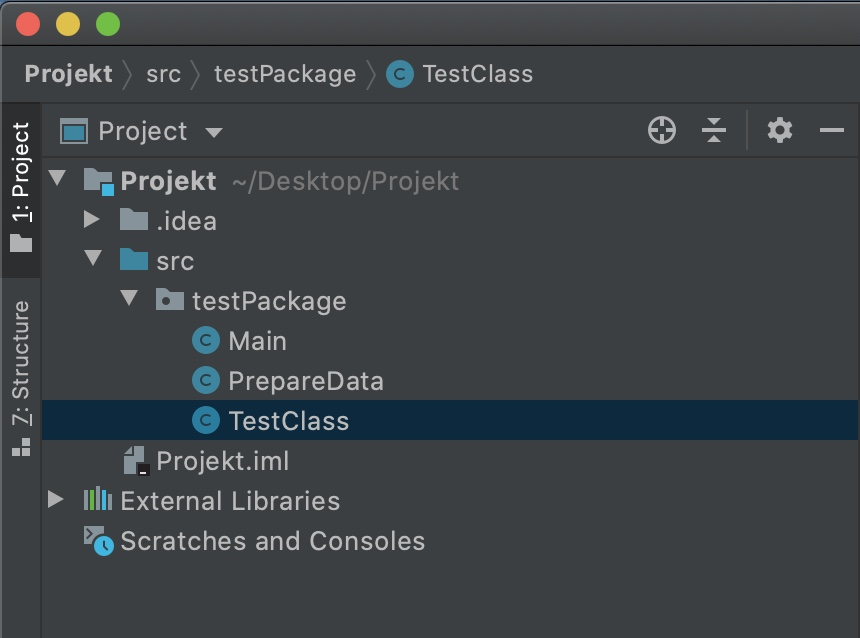
\includegraphics[width=\linewidth]{Images/img1.jpg}
  \caption{Darstellung eines Bahnhofs}
\end{figure}

\subsection{Tabelle}

\begin{table}[h]
\begin{center}
\begin{tabular}[h]{c|c|c}
ICE 1 & ICE 2 & ICE 3 \\ \hline
200 km/h & 250 km/h  & 300 km/h  \\
\end{tabular}
\caption{Sehr sehr schöne Tabelle}
\end{center}
\end{table} % implement chapter .tex file from the same folder
\newpage
\section{Berechnung des \Gls{fahrtverlauf}s} \label{kapitelFahrtverlauf}
Der \Gls{fahrtverlauf} eines Fahrzeuges wird bei der Berechnung auf zwei verschiedenen Arten gespeichert. Einmal in so genannten \textit{\$keyPoints}, welche in einem Array die Start- und Zielgeschwindigkeit (\textit{speed\_0} und \textit{speed\_1}), die Start- und Endposition (\textit{position\_0} und \textit{position\_1}) und die Start- und Endzeit (\textit{time\_0} und \textit{time\_1}) der einzelnen Beschleunigungen bzw. Verzögerungen abspeichern. Für die Überprüfung, ob ein Fahrzeug die zulässige Höchstgeschwindigkeit in einem \ac{infra} überschreitet, für die spätere Übermittlung der \Gls{echtzeitdaten} an das Fahrzeug und die exakte Positionsbestimmung, werden mittels der \textit{\$keyPoints} für jede Geschwindigkeitsänderungen (und bei \Gls{beharrungsfahrt}en in 1 Meter Abständen) unter anderem die aktuelle relative Position innerhalb eines \ac{infra}s (\textit{\$trainRelativePosition}), der \ac{infra} (\textit{\$trainSection}), die aktuelle Zeit (\textit{\$trainTimeChange}) und die aktuelle Geschwindigkeit (\textit{\$trainSpeedChange}) in gespeichert. 

Als Grundlage für die Berechnung des \Gls{fahrtverlauf}s werden zudem die Variablen \textit{\$indexCurrentSection} und \textit{\$indexTargetSection} benötigt, welche die Indexe der Start- und Ziel-\ac{infra}e in Bezug auf das Array \textit{\$next\_sections} beschreiben und die Arrays \textit{\$cumulativeSectionLengthStart} und \textit{\$cumulativeSectionLengthEnd}, welche für jeden \ac{infra} den Abstand zur aktuellen Position von dem Anfang und dem Ende des \ac{infra}s angeben.

Der \Gls{fahrtverlauf} wird mit der Funktion \textit{updateNextSpeed$($$)$} (\textit{functions\_fahrt\-ver\-lauf.php}) berechnet, welche als Parameter unter anderem die Zugdaten aus dem \textit{\$all\-Used\-Trains}-Array, Start- und Endzeit der Fahrt (\textit{\$startTime} und \textit{\$endTime}), den Ziel-\ac{infra} (\textit{\$targetSection}) und die relative Position in dem Ziel-\ac{infra} (\textit{\$targetPosition}) übergeben bekommt.
\begin{table}
\begin{center}
\renewcommand{\arraystretch}{1.2}
\begin{tabular}{c|c}
Bezeichnung & Funktion \\ \hline
\textit{\$keyPoint} (Array)                   			&   \makecell{Beschreibt eine Beschleunigung bzw.\\Verzögerung (\textit{position\_0}, \textit{position\_1},\\ \textit{time\_0}, \textit{time\_1}, \textit{speed\_0}, \textit{speed\_1})}           \\ \hline
\textit{\$next\_section} (Array)                  		&    IDs aller \ac{infra}e                  \\ \hline
\textit{\$next\_lenghts} (Array)                  		&    Längen aller \ac{infra}e                  \\ \hline
\textit{\$next\_v\_max} (Array)                  		&    Höchstgeschwindigkeit aller \ac{infra}e                  \\ \hline
\textit{\$indexCurrentSection} (Integer)             	&    Index des aktuellen \ac{infra}s               \\ \hline
\textit{\$indexTargetSection} (Integer)               	&    Index des Ziel-\ac{infra}s                  \\ \hline
\makecell{\textit{\$cumulativeSectionLengthStart}\\(Array) }	&    Absolute Startposition aller \ac{infra}e                  \\ \hline
\makecell{\textit{\$cumulativeSectionLengthEnd}\\(Array)  }	&    Absolute Endposition aller \ac{infra}e                  \\ \hline
\textit{\$trainPositionChange} (Array)                	&    Alle absoluten Positionen des \Gls{fahrtverlauf}s                  \\ \hline
\textit{\$trainSpeedChange} (Array)                  	&   Alle Geschwindigkeiten des \Gls{fahrtverlauf}s                  \\
\end{tabular}
\renewcommand{\arraystretch}{1}
\caption{Beschreibung der verwendeten Variablen für die \Gls{fahrtverlauf}sberechnung}
\label{table:vars}
\end{center}
\end{table}

In dem folgenden Abschnitt werden die einzelnen Schritte beschrieben, die durchlaufen werden, um den optimalen \Gls{fahrtverlauf} zu berechnen. In der Darstellung \ref{fig:fahrtverlauf} wird der Ablauf grob schematisch dargestellt.
\begin{figure}
\resizebox{1\textwidth}{!}{
\begin{tikzpicture}[node distance=1cm, auto]
\node[punkt] (a) {Berechnung bei einer Beschleunigung auf die maximal mögliche Geschwindigkeit};
\node[below=of a, punkt] (b) {Wird die Geschwindigkeit in \ac{infra}n überschritten?};
\node[right=of b, punkt](c) {Neuberechnung unter Berücksichtigung der Geschwindigkeitsüberschreitung};
\node[below=of b, punkt] (d) {Wird die Mindestzeit auf den \Gls{beharrungsfahrt}en eingehalten?};
\node[right=of d, punkt](e) {Neuberechnung unter Berücksichtigung der Mindestzeit auf einer Geschwindigkeit};
\node[below=of d, punkt] (f) {Erreicht der Fahrzeug mit einer Verspätung das Ziel?};
\node[right=of f, punkt] (g) {Kann die Geschwindigkeit reduziert werden, ohne dass das Fahrzeug eine Verspätung hat?};
\node[below=of f, punkt] (h) {Übermittlung der \Gls{echtzeitdaten} an das Fahrzeug};
\node[right=of g, punkt] (i) {Reduzierung der Geschwindigkeit unter Einhaltung der Ankunftszeit};
\node[right=of a, punkt] (j) {Ist eine Fahrt ohne Gefahrenbremsung möglich?};
\node[right=of j, punkt] (k) {Berechnung der Gefahrenbremsung};
\node[above=of j, punkt] (l) {Start der \Gls{fahrtverlauf}sberechnung};
\draw [pil] (a) -- (b);
\draw [pil] (b) --  node[pos=0.5] {Ja} (c);
\draw [pil] (c.north) -- +(0,0.4) -|  (b.north); 
\draw [pil] (b) -- node[pos=0.5,left] {Nein} (d);
\draw [pil] (d) --  node[pos=0.5] {Nein} (e);
\draw [pil] (e.north) -- +(0,0.3) -|  (d.north); 
\draw [pil] (d) -- node[pos=0.5,left] {Ja} (f);
\draw [pil] (f) -- node[pos=0.5] {Ja} (g);
\draw [pil] (f) -- node[pos=0.5,left] {Nein} (h);
\draw [pil] (g) -- node[pos=0.5] {Ja} (i);
\draw [pil] (g.south) -- node[pos=0.5,left] {Nein} +(0,-1) |-  (h.east); 
\draw [pil] (i.south) -- +(0,-1) |-  (h.east); 
\draw [pil] (j) -- node[pos=0.5,above] {Ja} (a);
\draw [pil] (j) -- node[pos=0.5] {Nein} (k);
\draw [pil] (l) -- (j);
\draw [pil] (k.east) -- +(0.5,0) |- (h.east);
\end{tikzpicture}
}
\caption{Ablaufplan der \Gls{fahrtverlauf}sberechnung}
\label{fig:fahrtverlauf}
\end{figure}
\subsection{Ermittlung der Start- und Endposition der einzelnen \ac{infra}e unter Berücksichtigung der Zuglänge}
Für die Berechnung eines exemplarischen \Gls{fahrtverlauf}s wurden die in Tabelle \ref{table:infraex} definierten \ac{infra}e verwendet. Diese \ac{infra}e wurden so gewählt, dass alle Funktionen und die Allgemeingültigkeit des Algorithmus gezeigt werden können und existieren in dieser Form im \ac{ebuef} nicht. 
\begin{table}
\begin{center}
\renewcommand{\arraystretch}{1.2}
\begin{tabular}{c| C{2cm} |c}
\ac{infra}s-ID & Länge & zulässige Höchstgeschwindigkeit \\ \hline
1000                   &   300 $m$    & 120 $km/h$                        \\ \hline
1001                  &    400 $m$   & 120 $km/h$                        \\ \hline
1002                   &   300 $m$    &        120 $km/h$                         \\ \hline
1003                   &    400 $m$   &         90 $km/h$                        \\ \hline
1004                   &    300 $m$   &            60 $km/h$                     \\ \hline
1005                   &   200 $m$    &           60 $km/h$                      \\ \hline
1006                   &  400 $m$     &      90 $km/h$                           \\ \hline
1007                   &  500 $m$     &      120 $km/h$                           \\ \hline
1008                   &   300 $m$    &      120 $km/h$                           \\ \hline
1009                   &   400 $m$    &      100 $km/h$                           \\ \hline
1010                   &   300 $m$    &      60 $km/h$                           \\ \hline
1011                   &   300 $m$    &         40 $km/h$                        \\ 
\end{tabular}
\renewcommand{\arraystretch}{1}
\caption{Exemplarische \ac{infra}e}
\label{table:infraex}
\end{center}
\end{table}
Als exemplarisch gewählte Zugdaten wurden die in Tabelle \ref{table:train-ex} definierten Daten verwendet.
\begin{table}[]
\begin{center}
\renewcommand{\arraystretch}{1.2}
\begin{tabular}{r L{3cm}}
relative Startposition                   &   10 $m$                         \\ 
relative Zielposition                  &    290 $m$                         \\ 
aktueller \ac{infra}                   &   1001                         \\ 
Ziel-\ac{infra}                  &    1010                         \\ 
Startgeschwindigkeit                   &   0 $km/h$                          \\ 
Zielgeschwindigkeit                   &    0 $km/h$                        \\ 
Zuglänge                   &    50 $m$                        \\ 
Bremsverzögerung                   &    0,8 $m/s^{2}$                        \\ 
Fahrplan vorhanden                   &    ja                        \\ 
Zeit bis zur nächsten Betriebsstelle                   &    210 $s$                        \\ 
\end{tabular}
\renewcommand{\arraystretch}{1}
\caption{Exemplarische Zugdaten}
\label{table:train-ex}
\end{center}
\end{table}

Die zuvor ermittelten nächsten \ac{infra}e inklusive derer Längen und zulässigen Höchstgeschwindigkeit müssen für die Berechnung des \Gls{fahrtverlauf}s angepasst werden, da ein Fahrzeug erst beschleunigen darf, wenn das komplette Fahrzeug in den \ac{infra} eingefahren ist. In Darstellung \ref{fig:it1} sind die \ac{infra}e dargestellt, wie sie von der Fahrzeugsteuerung ermittelt wurden. Dabei werden alle \ac{infra}e, die das Fahrzeug bereits durchfahren hat oder hinter dem Ziel-\ac{infra} liegen nicht dargestellt. Zudem wird in dem aktuellen \ac{infra} die relative Position von der Länge abgezogen und der Ziel-\ac{infra} wird nur bis zur relativen Zielposition abgebildet. Dementsprechend ist der erste \ac{infra} in der Darstellung \ref{fig:it1} der \ac{infra} mit der ID 1001. Dieser hat aufgrund der aktuellen relativen Position des Fahrzeugs eine Länge von 290 $m$. Und der letzte \ac{infra} ist der \ac{infra} mit der ID 1010 und einer Länge von ebenfalls 290 $m$.
\begin{figure}
  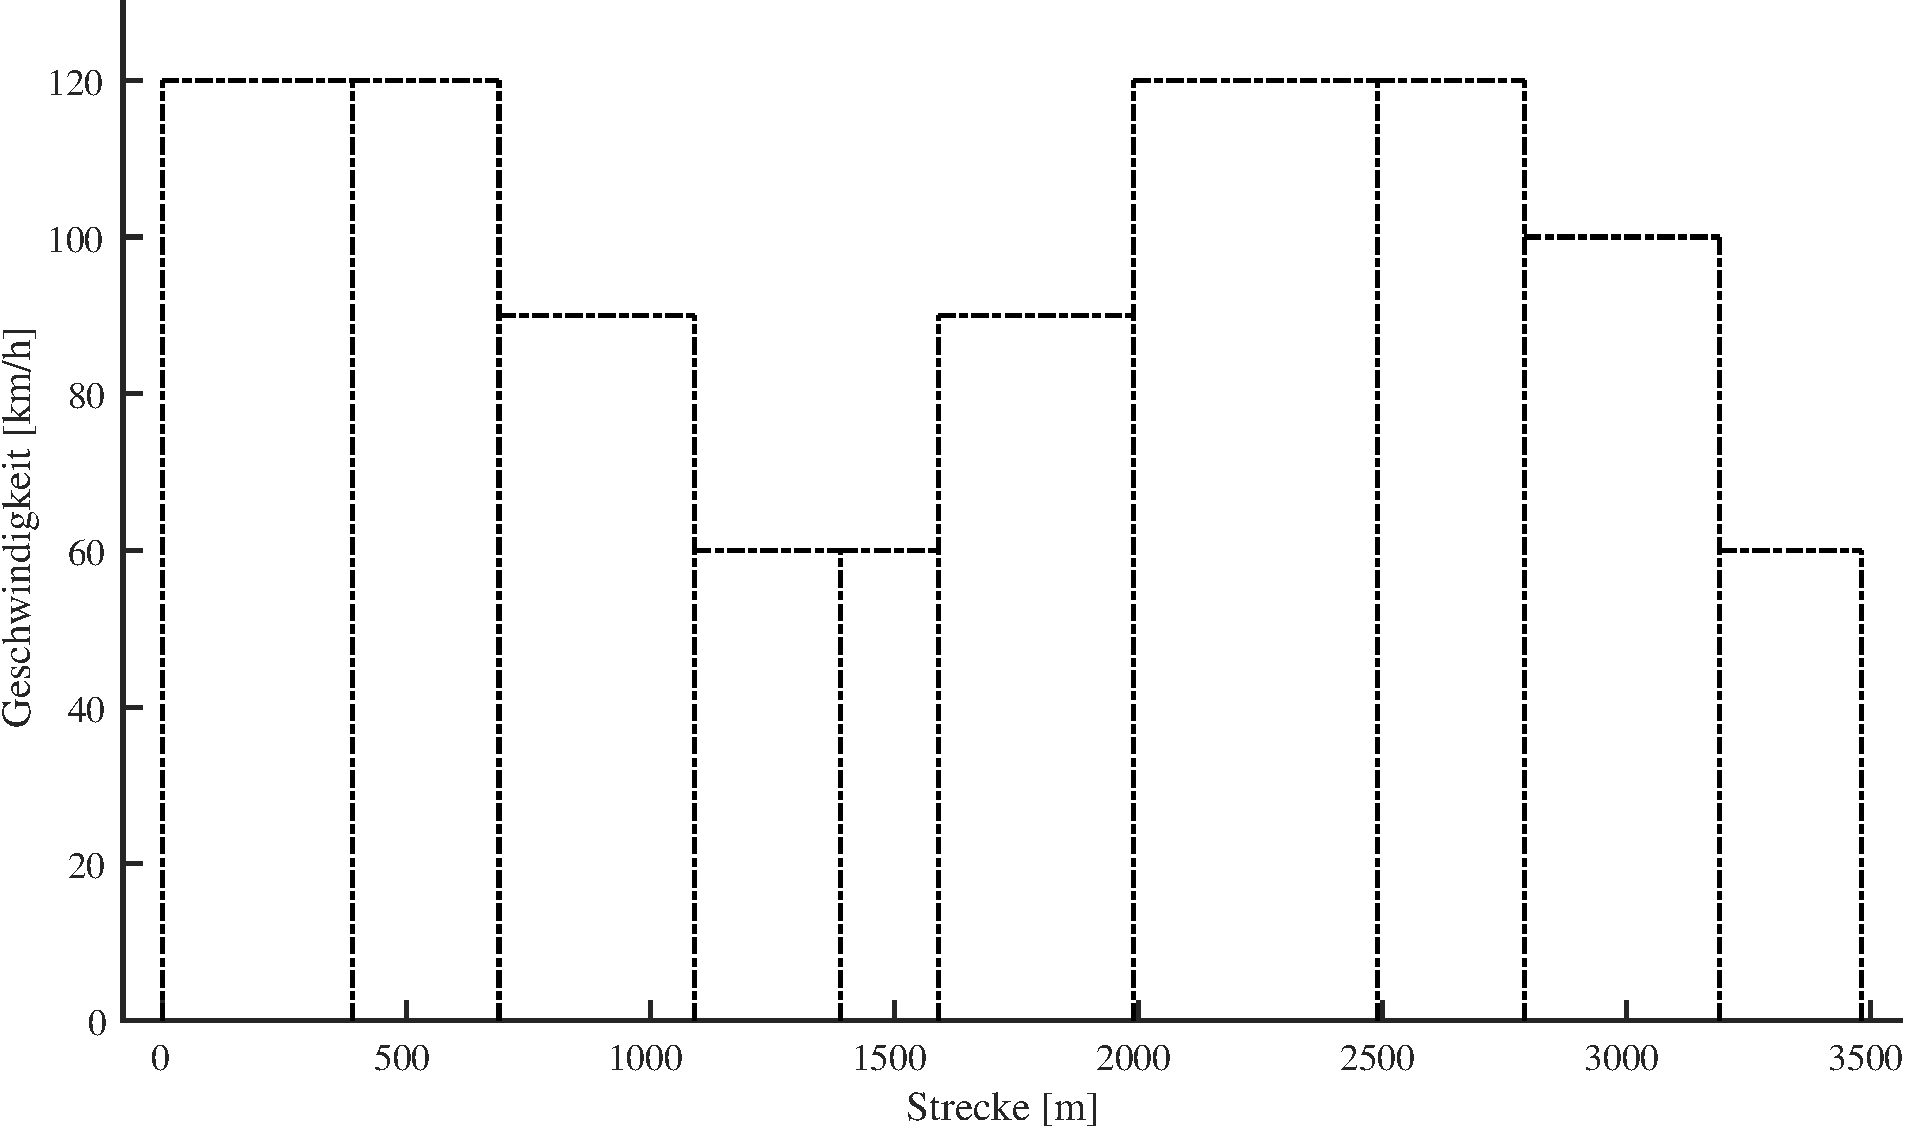
\includegraphics[width=\linewidth]{../images/matlab/it1.pdf}
  \caption{Infra-Abschnitte und die zugehörige Höchstgeschwindigkeit}
  \label{fig:it1}
\end{figure}

Bei der Berücksichtigung der Fahrzeuglänge wird mit einer \textit{for}-Schleife über alle \ac{infra}e iteriert und die Zuglänge auf die Länge das \ac{infra}s addiert. Von dieser neu ermittelten Endposition des \ac{infra}s wird überprüft, ob zwischen der vorherigen Endposition und der neu ermittelten Endposition ein \ac{infra} liegt, dessen zulässige Höchstgeschwindigkeit geringer ist, als die des ursprünglichen \ac{infra}s. Wenn dieser Fall eintritt, wird der \ac{infra} nur so weit verlängert, dass keine Höchstgeschwindigkeit der folgenden \ac{infra}e überschritten wird. Nach der Ermittlung der neuen Endposition, startet die \textit{for}-Schleife mit dem \ac{infra}, in dem sich die Endposition sich befindet. Sobald der Ziel-\ac{infra} erreicht wurde, wird die Schleife abgebrochen. Die neu ermittelten \ac{infra}e werden in den Arrays \textit{\$next\_lengths\_mod} und \textit{\$next\_v\_max\_mod} abgespeichert (analog zu den Arrays \textit{\$next\_lengths} und \textit{\$next\_v\_max}). 

Durch diesen Algorithmus kann es dazu kommen, dass sich die Anzahl der \ac{infra}e verändert hat, wodurch die \ac{infra}e nicht mehr eindeutig mit der Infrastruktur-ID bezeichnet werden können. Mittels \textit{\$next\_""lengths\_""mod} und \textit{\$next\_""v\_""max\_""mod} werden mit der Funktion \textit{create\-Cumulative\-Sec\-tions$($$)$} (\textit{func\-tions\_""fahrt\-ver\-lauf.php}) für jeden \ac{infra} die absolute Start- und Endposition in den Arrays \textit{\$cumulative\-Section\-Length\-Start\-Mod} und \textit{\$cumulativeSectionLengthEndMod} gespeichert. Diese Umwandlung ist essentiell für die Überprüfung, in welchem \ac{infra} ein Fahrzeug sich aktuell befindet. Die neu berechneten \ac{infra}e sind in der Darstellung \ref{fig:it2} in rot abgebildet und beschreiben die maximale Geschwindigkeit, die ein Fahrzeug an der jeweiligen Position fahren darf.
\begin{figure}
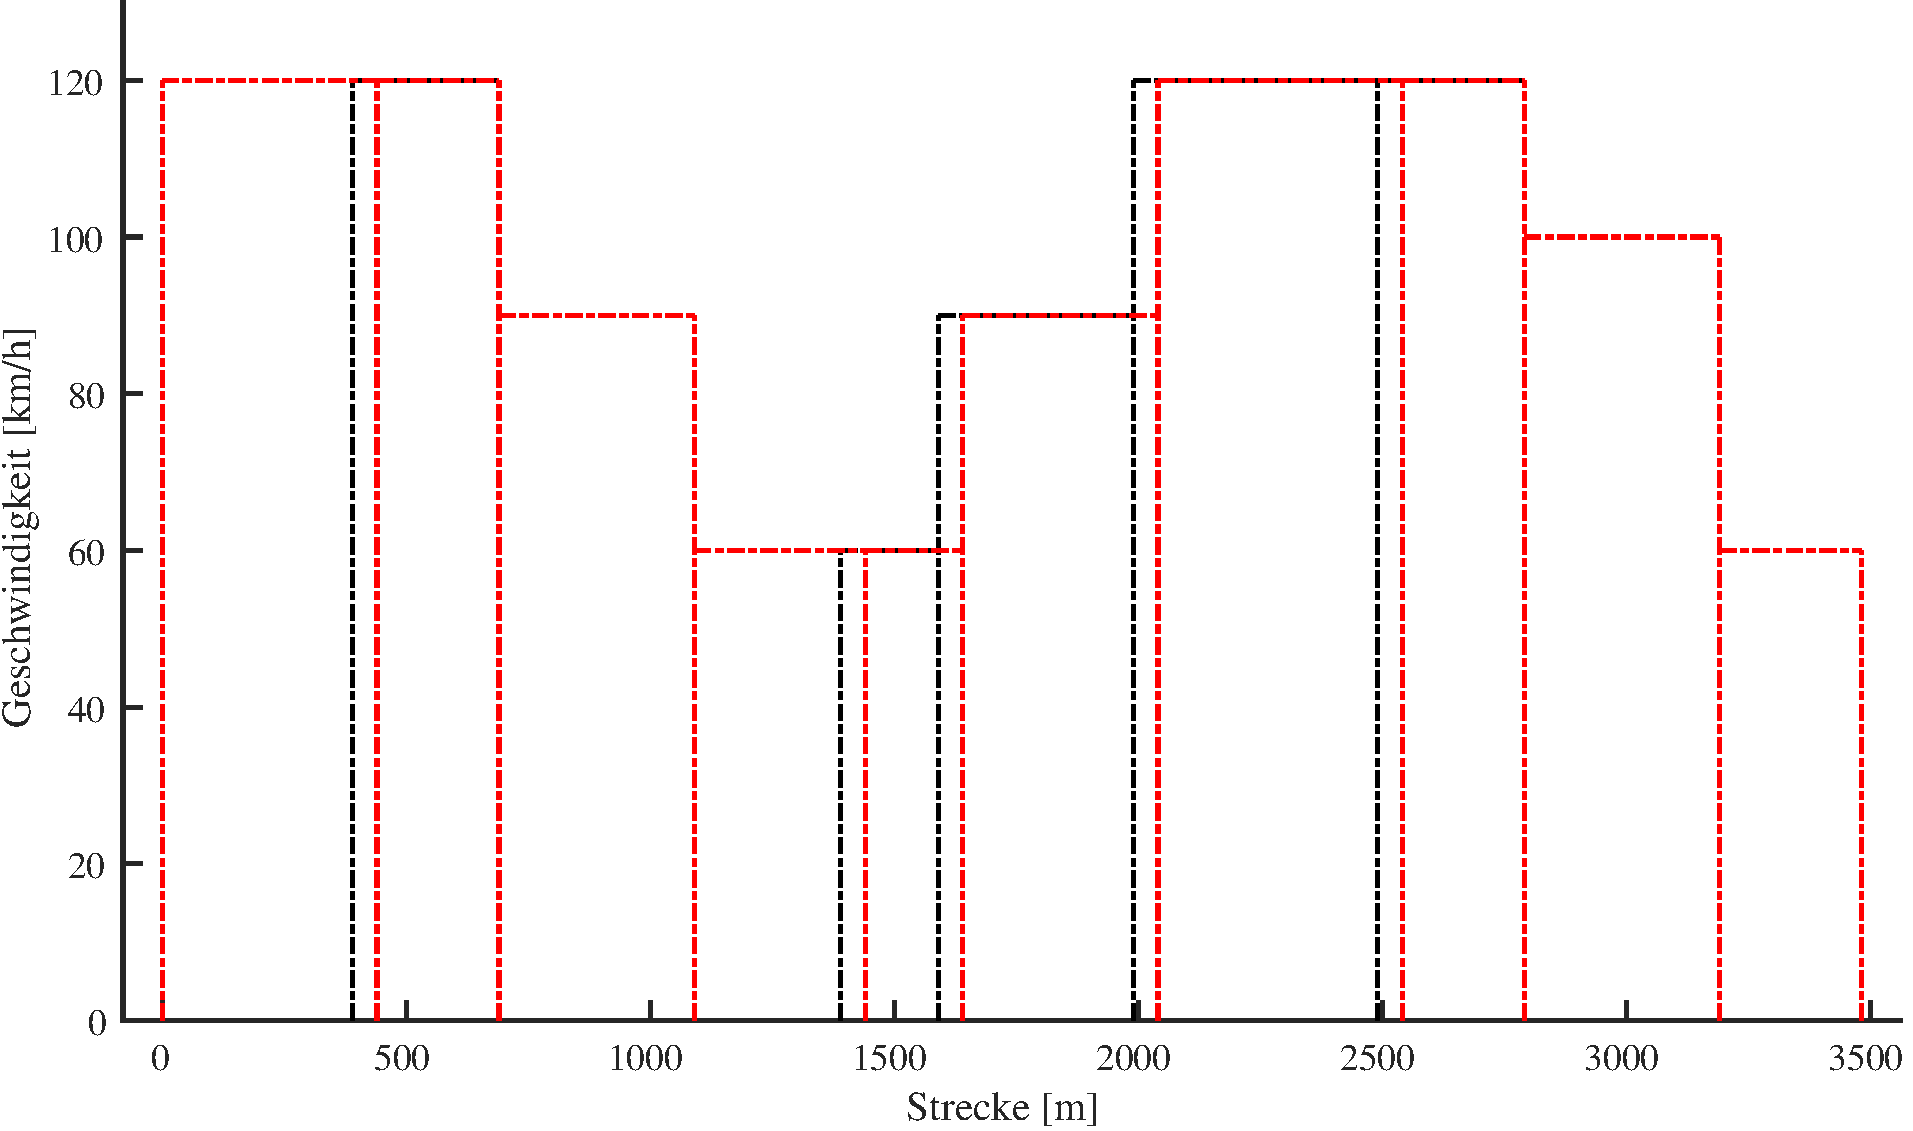
\includegraphics[width=\linewidth]{../images/matlab/it2.pdf}
\caption{Infra-Abschnitte und die zugehörige Höchstgeschwindigkeit unter Berücksichtigung der Fahrzeuglänge}
\label{fig:it2}
\end{figure}
\subsection{Berechnung bei einer Beschleunigung auf die maximal mögliche Geschwindigkeit} \label{v_max}
Im ersten Schritt der \Gls{fahrtverlauf}sberechnung wird die Distanz zwischen der aktuellen Position und der Ziel-Position mittels \textit{\$cumulativeSectionLengthStart}, \textit{\$cumulativeSectionLengthEnd}, \textit{\$indexCurrentSection} und \textit{\$indexTargetSection} berechnet. Für die Distanz und die Startgeschwindigkeit wird mit Hilfe der Funktion \textit{get\-V\-Max\-Be\-tween\-Two\-Points$($$)$} (\textit{func\-tions\_fahrt\-ver\-lauf.php}) (Code-Beispiel \ref{lst:getVMaxBetweenTwoPoints}) die maximale Geschwindigkeit ermittelt, auf die das Fahrzeug beschleunigen kann, um bis zum Ziel rechtzeitig bremsen zu können. Dabei wird in 10 $km/h$-Schritten iteriert und der maximale Wert zurückgegeben. Innerhalb der Funktion wir die Funktion \textit{getBrakeDistance$($$)$} (\textit{functions\_math.php}) (Code-Beispiel \ref{lst:getBrakeDistance}) aufgerufen, welche die benötigte Distanz für eine Beschleunigung bzw. Verzögerung berechnet und auf der Gleichung \ref{eq:s_v_ges} aus Kapitel \ref{formulaBeschleunigung} basiert.
\begin{figure}
\begin{lstlisting}[caption={\textit{getVMaxBetweenTwoPoints$($$)$} (\textit{functions\_fahrtverlauf.php})},captionpos=b,label={lst:getVMaxBetweenTwoPoints}]
// Ermittelt die maximale Geschwindigkeit zwischen zwei Punkten
function getVMaxBetweenTwoPoints(float $distance, int $v_0, int $v_1) {

	global $verzoegerung;
	global $globalFloatingPointNumbersRoundingError;

	$v_max = array();

	for ($i = 0; $i <= 120; $i = $i + 10) {
		if ((getBrakeDistance($v_0, $i, $verzoegerung) + getBrakeDistance($i, $v_1, $verzoegerung)) < ($distance + $globalFloatingPointNumbersRoundingError)) {
			array_push($v_max, $i);
		}
	}

	if (sizeof($v_max) == 0) {
		if ($v_0 == 0 && $v_1 == 0 && $distance > 0) {
			echo "Der zug müsste langsamer als 10 km/h fahren, um das Ziel zu erreichen.";
		} else {
			//emergencyBreak($id);
		}
	} else {
		if ($v_0 == $v_1 && max($v_max) < $v_0) {
			$v_max = array($v_0);
		}
	}

	return max($v_max);
}
\end{lstlisting}
\end{figure}

Durch die gegebene Startgeschwindigkeit und die größtmögliche Geschwindigkeit wird ein erster \Gls{fahrtverlauf} berechnet, wobei zwei \textit{\$keyPoints} erzeugt werden. Mithilfe der Funktion \textit{createTrainChanges$($$)$} (\textit{functions\_fahrtverlauf.php}) wird aus diesen beiden \textit{\$keyPoints} für jede Geschwindigkeitsveränderung die aktuelle absolute Position und Geschwindigkeit ermittelt. An den Positionen, an denen das Fahrzeug eine konstante Geschwindigkeit hat, wird in 1 Meter Abständen die absolute Position und die Geschwindigkeit gespeichert. Die ermittelten Daten werden in den Arrays \textit{\$trainPositionChange} und \textit{\$trainSpeedChange} gespeichert und sind in der Darstellung \ref{fig:it3} abgebildet.
\begin{figure}
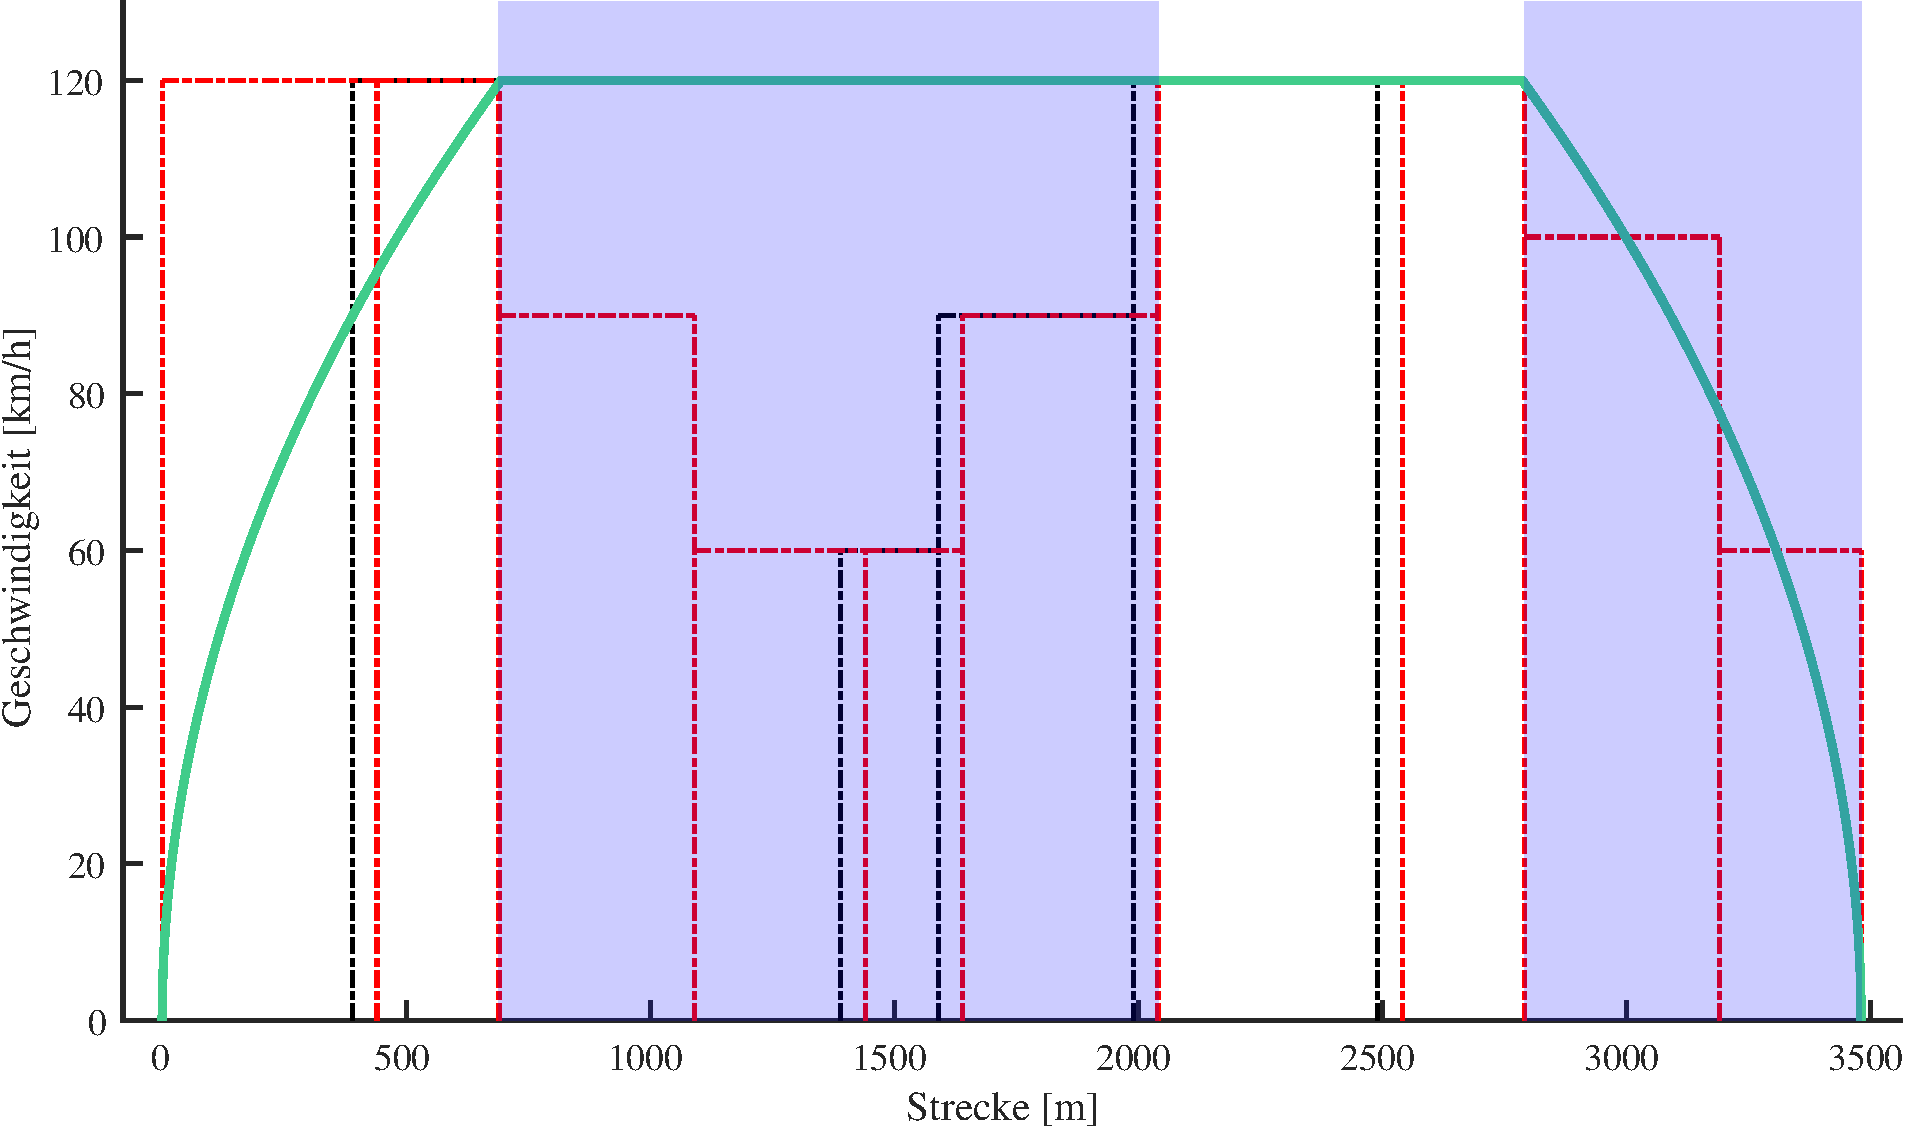
\includegraphics[width=\linewidth]{../images/matlab/it3.pdf}
\caption{\Gls{fahrtverlauf}sberechnung (1. Iterationsschritt)}
\label{fig:it3}
\end{figure}
\subsection{Überprüfung des \Gls{fahrtverlauf}s nach Geschwindigkeitsüberschreitungen} \label{überprüfung}
Für die Überprüfung, ob es bei einem \Gls{fahrtverlauf} zu einer Überschreitung der zulässigen Höchstgeschwindigkeit kommt, wird nach jeder Berechnung die Funktion \textit{check\-If\-Train\-Is\-To\-Fast\-In\-Certain\-Sec\-tions$($$)$} (\textit{functions\_fahrtverlauf.php}) (Code-Beispiel \ref{lst:checkIfTrainIsToFastInCertainSections}) aufgerufen. In dieser Funktion wird über alle absoluten Positionen (\textit{\$trainPositionChange}) iteriert, überprüft in welchem \ac{infra} sich diese Position befindet und überprüft, ob die zugehörige Geschwindigkeit aus dem \textit{\$trainSpeedChange}-Array die zulässige Höchstgeschwindigkeit überschreitet. Sobald in einem \ac{infra} eine Geschwindigkeitsüberschreitung vorliegt, wird der zugehörige Index des \ac{infra}s in dem \textit{\$faildSections}-Array gespeichert. Diese \ac{infra}e sind in der Darstellung \ref{fig:it3} Lila hinterlegt. 

Als Rückgabewert der Funktion wird ein Array zurückgegeben, welches abspeichert, ob und in welchen \ac{infra}en es zu einer Geschwindigkeitsüberschreitung gekommen ist (\textit{failed} und \textit{failed\_""sec\-tions}).
\begin{figure}
\begin{lstlisting}[caption={\textit{checkIfTrainIsToFastInCertainSections$($$)$} (\textit{func\-tions\_""fahrt\-ver\-lauf\-.php})},captionpos=b,label={lst:checkIfTrainIsToFastInCertainSections}]
// Überprüft, ob das Fahrzeug in Infra-Abschnitten die zulässige
// Höchstgeschwindigkeit überschreitet
function checkIfTrainIsToFastInCertainSections() {

	global $trainPositionChange;
	global $trainSpeedChange;
	global $cumulativeSectionLengthStartMod;
	global $next_v_max_mod;
	global $indexTargetSectionMod;

	$faildSections = array();

	foreach ($trainPositionChange as $trainPositionChangeKey => $trainPositionChangeValue) {
		foreach ($cumulativeSectionLengthStartMod as $cumulativeSectionLengthStartKey => $cumulativeSectionLengthStartValue) {
			if ($trainPositionChangeValue < $cumulativeSectionLengthStartValue) {
				if ($trainSpeedChange[$trainPositionChangeKey] > $next_v_max_mod[$cumulativeSectionLengthStartKey - 1]) {
					array_push($faildSections, ($cumulativeSectionLengthStartKey -1));
				}

				break;
			} else if ($cumulativeSectionLengthStartKey == $indexTargetSectionMod) {
				if ($trainPositionChangeValue > $cumulativeSectionLengthStartValue) {
					if ($trainSpeedChange[$trainPositionChangeKey] > $next_v_max_mod[$cumulativeSectionLengthStartKey]) {
						array_push($faildSections, $cumulativeSectionLengthStartKey);
					}

					break;
				}
			}
		}
	}

	if (sizeof($faildSections) == 0) {
		return array("failed" => false);
	} else {
		return array("failed" => true, "failed_sections" => array_unique($faildSections));
	}
}
\end{lstlisting}
\end{figure}
\subsection{Neuberechnung unter Berücksichtigung der Geschwindigkeitsüber-\\schreitung} \label{neuberechnung}
In dem Fall, dass es zu einer Geschwindigkeitsüberschreitung gekommen ist, wird der \Gls{fahrtverlauf} neu berechnet. Als Grundlage dafür dienen die \textit{failed\_sections} aus der \textit{check\-If\-Train\-Is\-To\-Fast\-In\-Certain\-Sections$($$)$}-Funktion (\textit{functions\_fahrtverlauf.php}) (Code-Beispiel \ref{lst:checkIfTrainIsToFastInCertainSections}). Die Funktion \textit{recalculate\-Key\-Points$($$)$} (\textit{functions\_fahrtverlauf.php}) vergleicht dabei immer zwei benachbarte \textit{\$keyPoints} und berechnet in dem Fall einer Geschwindigkeitsüberschreitung mit der Funktion \textit{check\-Between\-Two\-Key\-Points$($$)$} (\textit{func\-tions\_fahrt\-ver\-lauf\-.php}) diese neu. In dem Fall, dass zwischen zwei benachbarten \textit{\$keyPoints} die zulässige Höchst\-ge\-schwin\-dig\-keit überschritten wird, wird die absolute Start- und End-Position dieser Ge\-schwin\-digkeits\-über\-schrei\-tung gespeichert. 

In dem fol\-gen\-den Schritt wird wie in dem Abschnitt \ref{v_max} zwischen den Start-Werten des ersten \textit{\$keyPoints} und der ersten Geschwindigkeitsüberschreitung die maximale Geschwindigkeit berechnet und zwei neue \textit{\$keyPoints} erzeugt. Das gleiche passiert zwischen der Position der letzten Geschwindigkeitsüberschreitung und den End-Werten des zweiten \textit{\$keyPoints}. Dadurch wird sichergestellt, dass immer eine gerade Anzahl an \textit{\$keyPoints} existiert und somit in jedem Iterationsschritt zwei benachbarte \textit{\$keyPoints} verglichen werden können. Nachdem alle \textit{\$keyPoint}-Paare überprüft wurden, werden mit Hilfe der \textit{create\-Train\-Changes$($$)$}-Funktion (\textit{functions\_fahrtverlauf.php}) die Arrays \textit{\$train\-Position\-Change} und \textit{\$train\-Speed\-Change} erzeugt. Der neu berechnete \Gls{fahrtverlauf} wird erneut der Funktion \textit{check\-If\-Train\-Is\-To\-Fast\-In\-Certain\-Sections$($$)$} (\textit{func\-tions\_""fahrt\-ver\-lauf\-.php}) (Code-Bei\-spiel \ref{lst:checkIfTrainIsToFastInCertainSections}) übergeben. Dieser Prozess wird solange durchlaufen, bis es zu keiner Geschwindigkeitsüberschreitung mehr kommt. In den folgenden Abbildungen (Darstellung \ref{fig:it4}, \ref{fig:it5} und \ref{fig:it6}) werden die Ergebnisse der einzelnen Iterationsschritte visuell abgebildet, wobei die grau gepunkteten Linien die Ergebnisse der vorherigen Iterationsschritte darstellen.
\begin{figure}
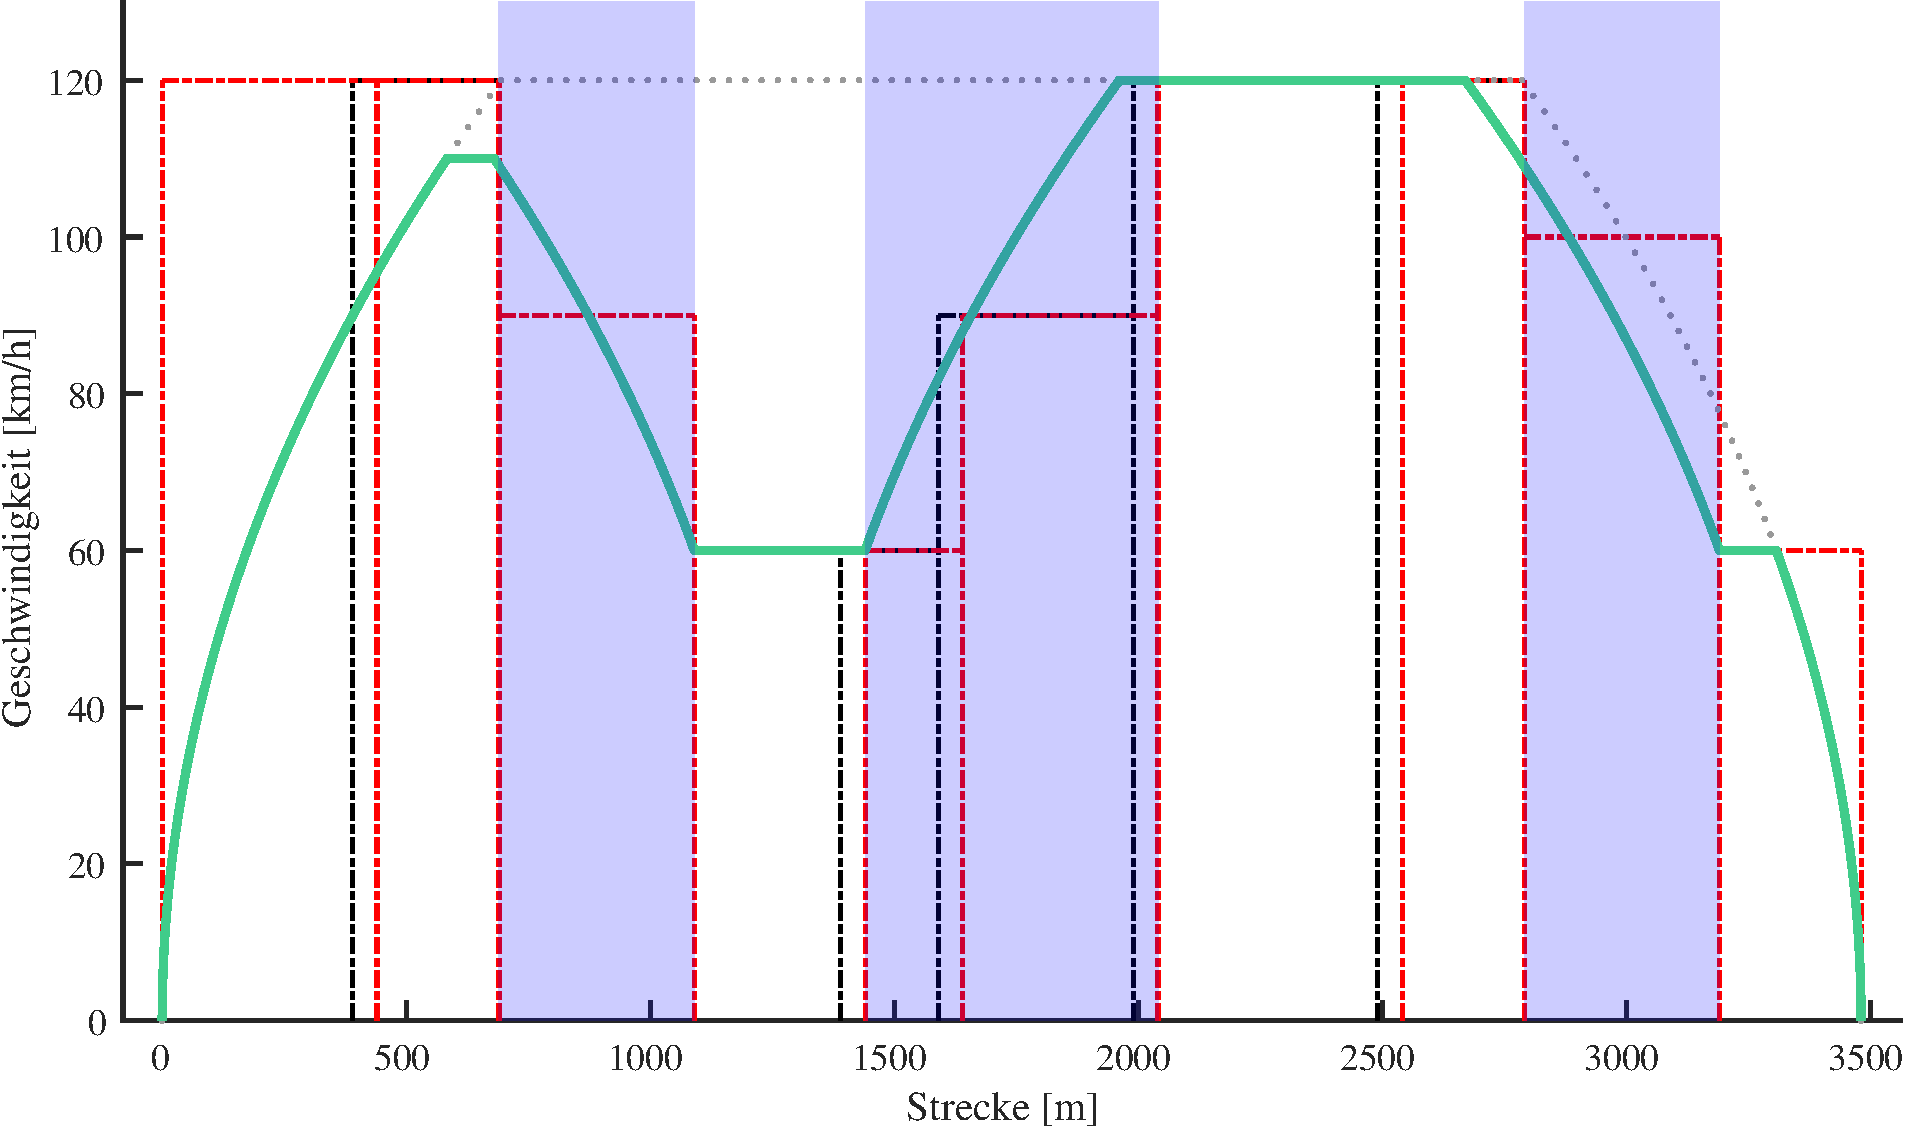
\includegraphics[width=\linewidth]{../images/matlab/it4.pdf}
\caption{\Gls{fahrtverlauf}sberechnung (2. Iterationsschritt)}
\label{fig:it4}
\end{figure}
\begin{figure}
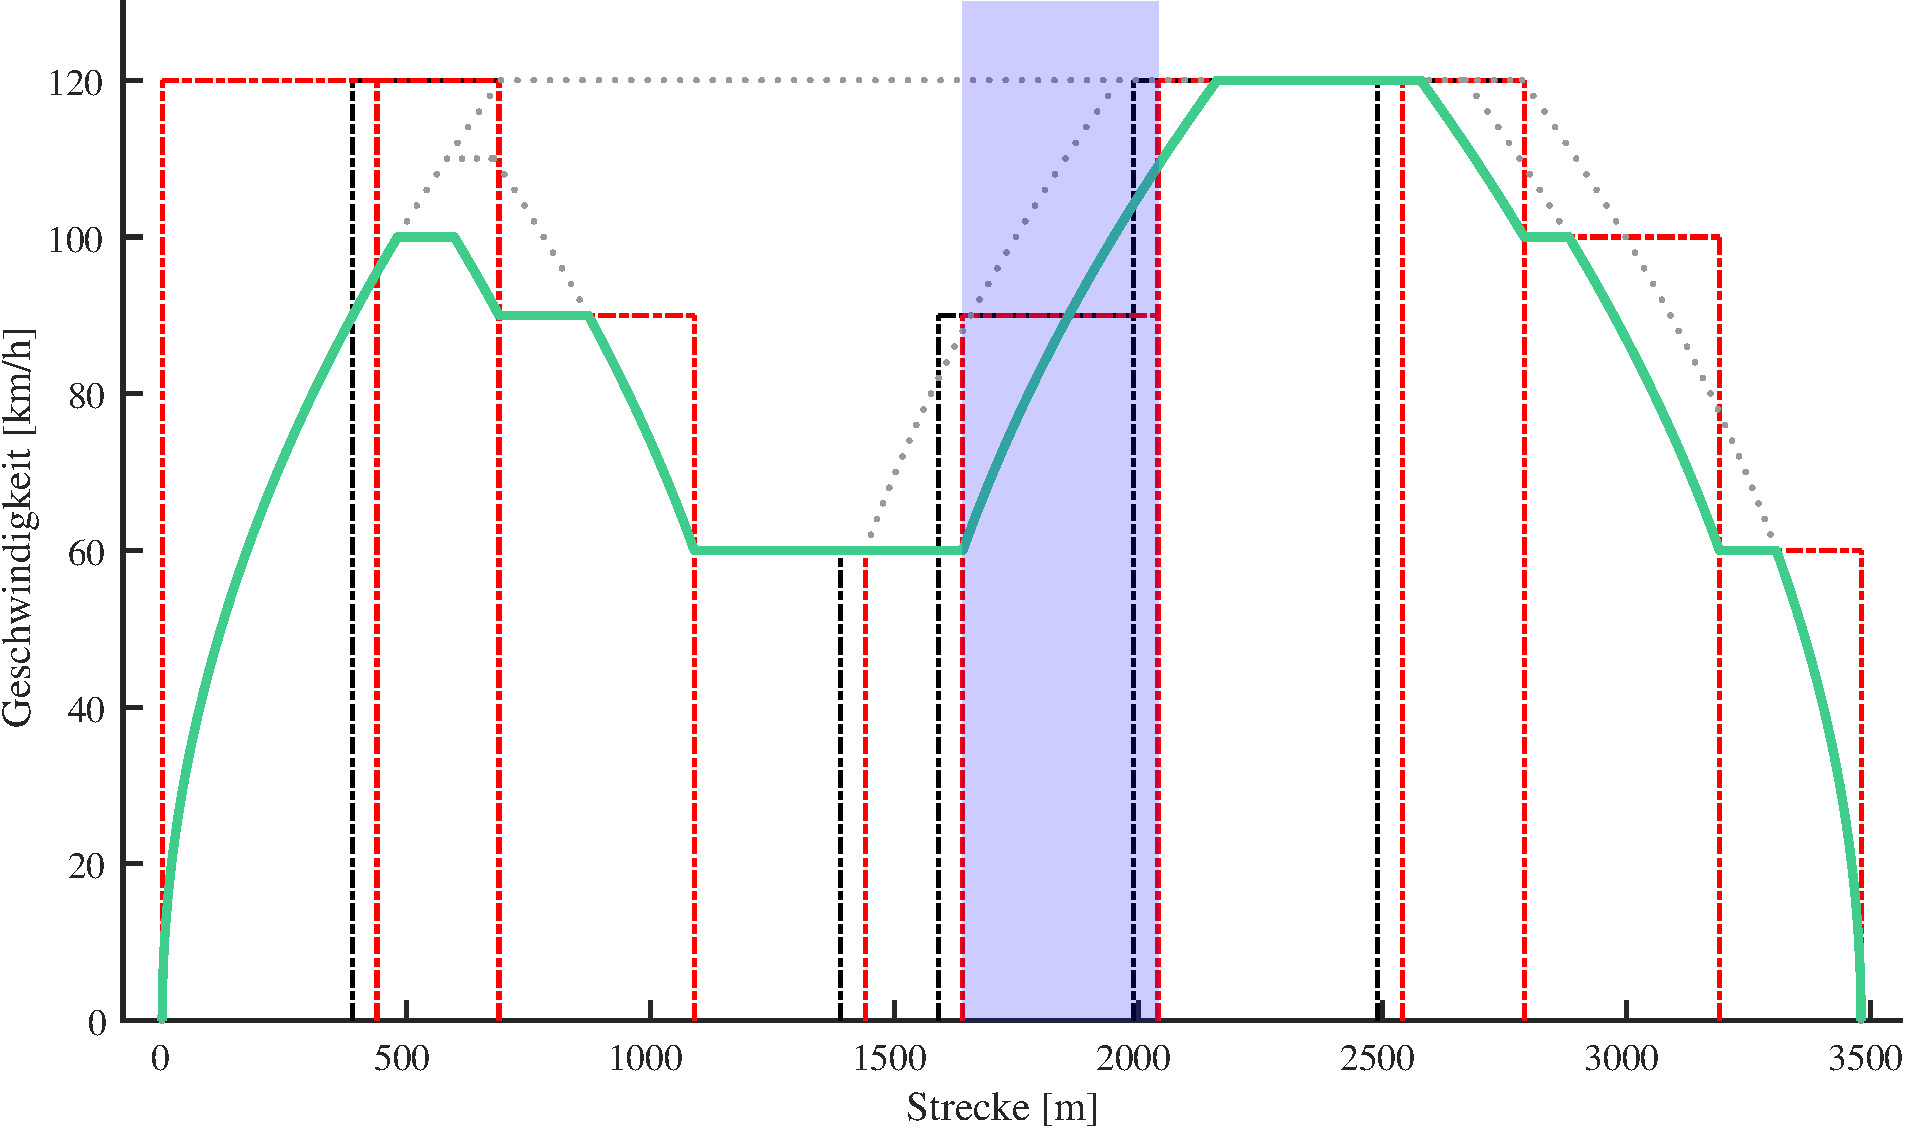
\includegraphics[width=\linewidth]{../images/matlab/it5.pdf}
\caption{\Gls{fahrtverlauf}sberechnung (3. Iterationsschritt)}
\label{fig:it5}
\end{figure}
\begin{figure}
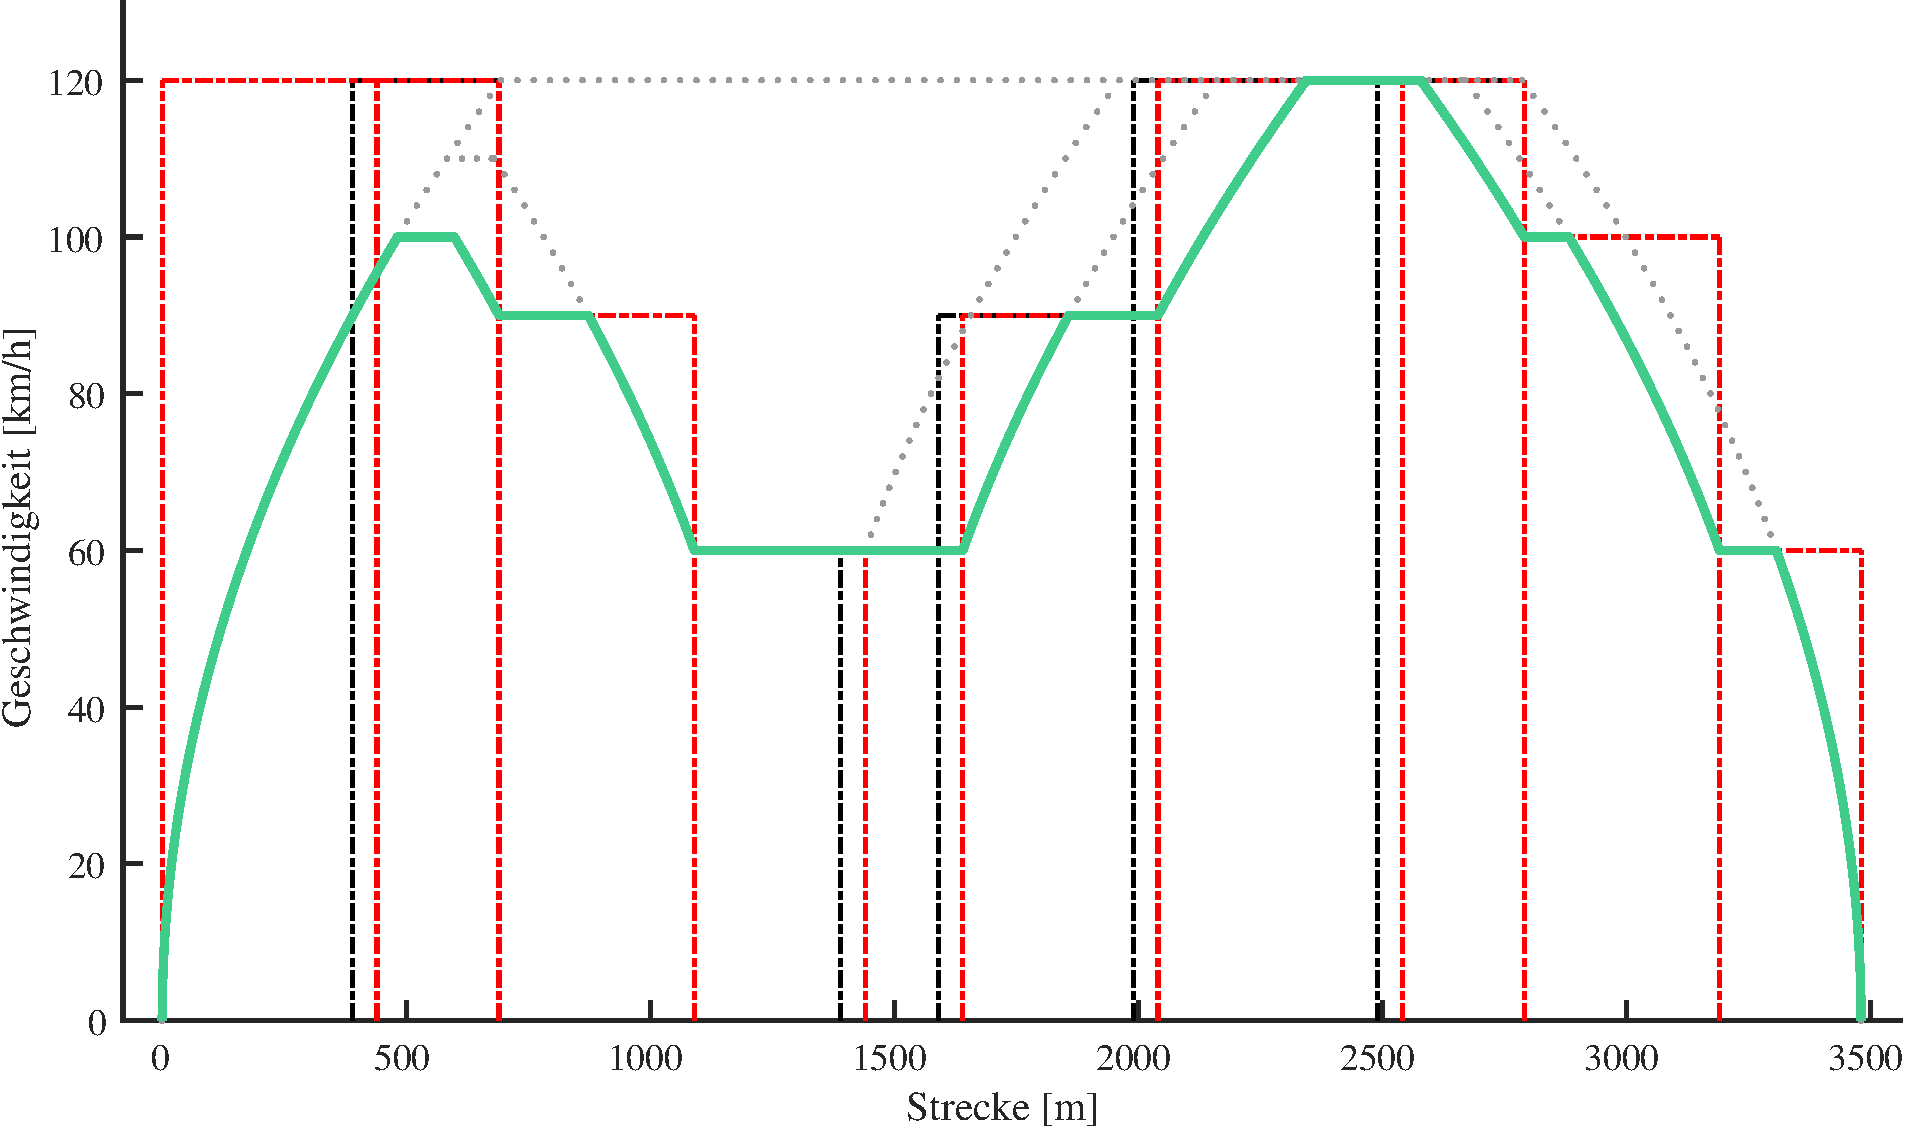
\includegraphics[width=\linewidth]{../images/matlab/it6.pdf}
\caption{\Gls{fahrtverlauf}sberechnung (4. Iterationsschritt)}
\label{fig:it6}
\end{figure}
\subsection{Einhaltung der Mindestzeit auf einer \Gls{beharrungsfahrt}} \label{minTime}
Für eine möglichst realitätsnahe Simulation kann über die Variable \textit{\$global\-Time\-On\-One\-Speed} in der Datei \textit{global\_variables.php} eine Mindestzeit festgelegt werden, die ein Fahrzeug auf einer Geschwindigkeit mindestens einhalten muss (\Gls{beharrungsfahrt}). Ebenfalls kann über die Variablen \textit{\$useMinTimeOnSpeed} und \textit{\$errorMinTimeOnSpeed} festgelegt werden, ob die Funktion aktiviert sein soll und ob es in dem Fall, dass diese Zeit nicht eingehalten werden kann, zu einer Fehlermeldung kommen soll. Im Falle einer Fehlermeldung würde das Fahrzeug nicht losfahren bzw. eine Gefahrenbremsung einleiten, falls das Fahrzeug aktuell eine Geschwindigkeit $v > 0$ $km/h$ hat. 

Wenn auf einem Abschnitt die Mindestzeit nicht eingehalten werden kann, kann eine Beschleunigung später eingeleitet werden, eine Verzögerung vorzeitiger eingeleitet werden oder auf eine kleinere Geschwindigkeit beschleunigt werden. Dadurch, dass sich eine Verschiebung einer Beschleunigung bzw. Verzögerung auf die nächsten Abschnitte auswirken kann, wird der \Gls{fahrtverlauf} in \textit{\$subsections} unterteilt. Eine \textit{\$subsection} beschreibt dabei den Bereich des \Gls{fahrtverlauf}s, in dem das Fahrzeug zum ersten Mal beschleunigt und zum letzten Mal abbremst. In der Darstellung \ref{fig:it7} wurde der exemplarische \Gls{fahrtverlauf} somit in zwei \textit{\$subsection} unterteilt, welche Lila bzw. Gelb hinterlegt sind.
\begin{figure}
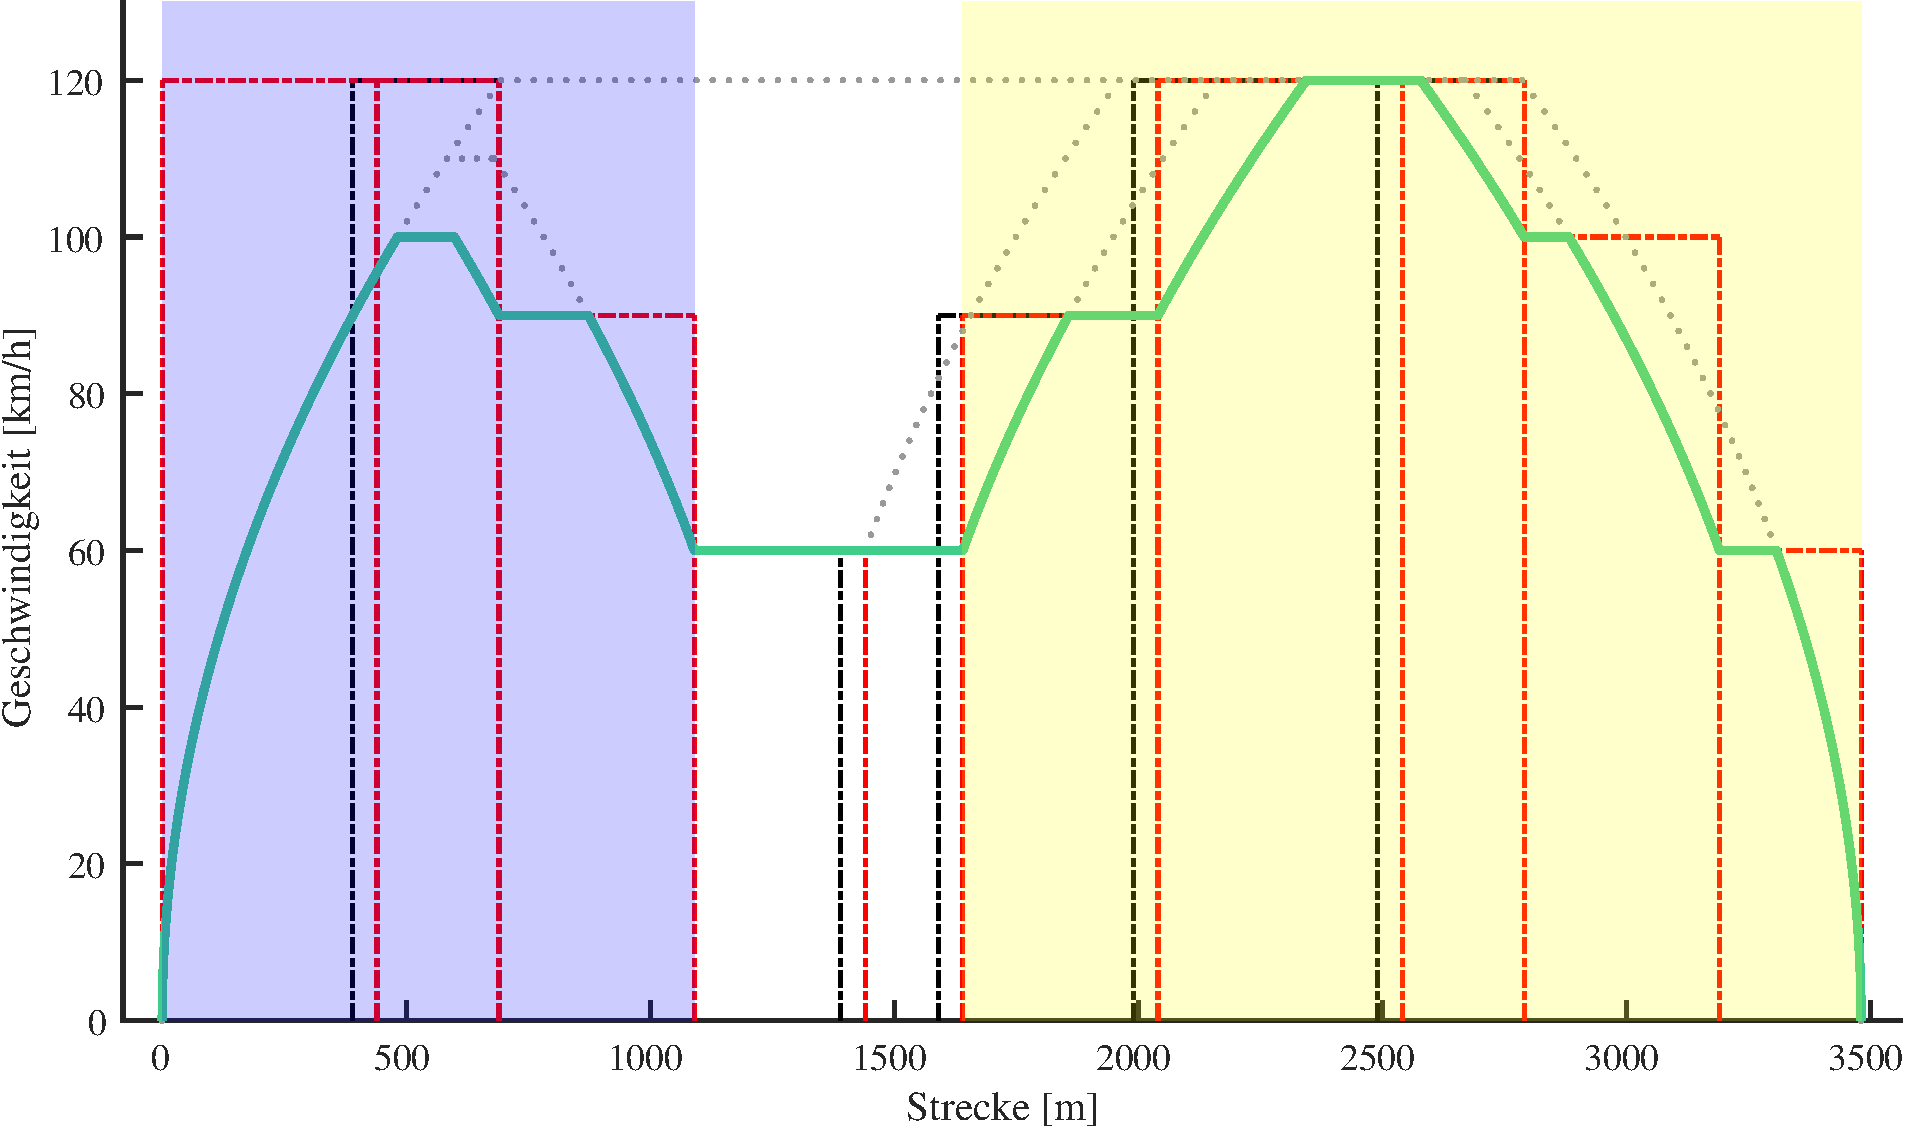
\includegraphics[width=\linewidth]{../images/matlab/it7.pdf}
\caption{Einteilung des \Gls{fahrtverlauf}s in \textit{\$subsections}}
\label{fig:it7}
\end{figure}
Durch diese Einteilung kann verhindert werden, dass es zu Konflikten kommt. Falls die Beschleunigungen bzw. Verzögerungen soweit nach hinten bzw. nach vorne verschoben werden müssen, kann die maximale Geschwindigkeit auf dieser \textit{\$subsection} reduziert werden und die zur Verfügung stehende Strecke vergrößert werden. Wie in Darstellung \ref{fig:it7} zu erkennen wird hierbei im ersten Schritt der Abschnitt zwischen zwei \textit{\$subsections} ausgelassen. Nach der Ermittlung der \textit{\$subsections} wird überprüft, ob auf den Abschnitten zwischen den \textit{\$subsections} die Mindestzeit eingehalten wird. Wenn das nicht der Fall ist, wird der Abschnitt automatisch der in Fahrtrichtung hinteren \textit{\$subsection} zugeordnet. Dadurch wird sichergestellt, dass das Fahrzeug, wenn es an einer Stelle des \Gls{fahrtverlauf}s die Geschwindigkeit reduziert, dies möglichst spät tut.

Nachdem die \textit{\$subsections} mittels der Funktion \textit{createSubsections$($$)$} (\textit{func\_tions\_""fahrt\-ver\-lauf.php}) erstellt wurden und mit der Funktion \textit{array\_reverse$($$)$} in umgekehrter Reihenfolge in dem Array \textit{\$subsection\_list} gesammelt wurden, wurde für jede \textit{\$subsection} ein Array erzeugt, welches die Variablen aus Tabelle \ref{table:subsection} beinhaltet und jede \textit{\$subsection} eindeutig beschreibt.
\begin{table}
\begin{center}
\renewcommand{\arraystretch}{1.2}
\begin{tabular}{c|c}
Index & Funktion \\ \hline
\textit{max\_index}                 	&  	\makecell{Index des \textit{\$keyPoints} mit der Beschleunigung auf die\\maximale Geschwindigkeit in der \textit{\$subsection}}     \\ \hline
\textit{indexes} (Array)                 		&    	Indexe aller beinhalteten \textit{\$keyPoints}                  \\ \hline
\makecell{\textit{is\_prev\_section}\\(Boolescher Wert)}           	&   	Berücksichtigung des Abschnitts vor der \textit{\$subsection}     \\ \hline
\makecell{\textit{is\_next\_section}\\(Boolescher Wert)}           	&     	Berücksichtigung des Abschnitts nach der \textit{\$subsection}                 \\ \hline
\textit{failed} (Boolescher Wert)             & Unterschreitung der Mindestzeit auf der \textit{\$subsection}     \\ 
\end{tabular}
\renewcommand{\arraystretch}{1}
\caption{Aufbau des \textit{\$subsection}-Arrays}
\label{table:subsection}
\end{center}
\end{table}

Bei den \textit{\$subsections}, bei denen die Mindestzeit für die \Gls{beharrungsfahrt}en nicht eingehalten wird (\textit{failed} == \textit{true}), wird überprüft, ob eine Verschiebung der Beschleunigungen bzw. Verzögerungen möglich ist. Bei der Verschiebung einer Beschleunigung bzw. Verzögerung wird die Differenz zwischen der Mindestzeit einer \Gls{beharrungsfahrt} (\textit{\$global\-Time\-On\-One\-Speed}) und der Zeit der vorherigen bzw. folgenden \Gls{beharrungsfahrt} berechnet und die Beschleunigung bzw. Verzögerung um diese Differenz verschoben.

Sollte bei einer Verschiebung die \textit{position\_1} eines \textit{\$keyPoints} hinter \textit{position\_0} des folgenden \textit{\$keyPoints} liegen (bei einer Beschleunigung), wird der zweite \textit{\$keyPoint} gelöscht und die Zielgeschwindigkeit des zweiten \textit{\$keyPoints} wird der Zielgeschwindigkeit des ersten \textit{\$keyPoints} zugewiesen. Gleiches geschieht bei der Verzögerung in umgekehrter Reihenfolge. 

Nach der Verschiebung wird überprüft, ob auf allen konstanten Geschwindigkeit die Mindestzeit eingehalten wird. Wenn das der Fall ist, wird die nächste \textit{\$subsection} überprüft. In dem Fall, dass durch die Verschiebung die Mindestzeit nicht eingehalten werden kann, wird die maximale Geschwindigkeit auf dieser \textit{\$subsection} um 10 $km/h$ reduziert, die \textit{\$subsections} neu berechnet und erneut über alle \textit{\$subsection} iteriert. Die Neuberechnung ist notwendig, da durch die Reduzierung der Geschwindigkeit die \textit{\$subsections} anders aufgeteilt sein können.

Wenn alle \textit{\$subsections} die Mindestzeit einhalten, wird der Algorithmus beendet. In der Darstellung \ref{fig:it9} ist der \Gls{fahrtverlauf} unter Einhaltung der Mindestzeit auf einer Geschwindigkeit abgebildet.
\begin{figure}
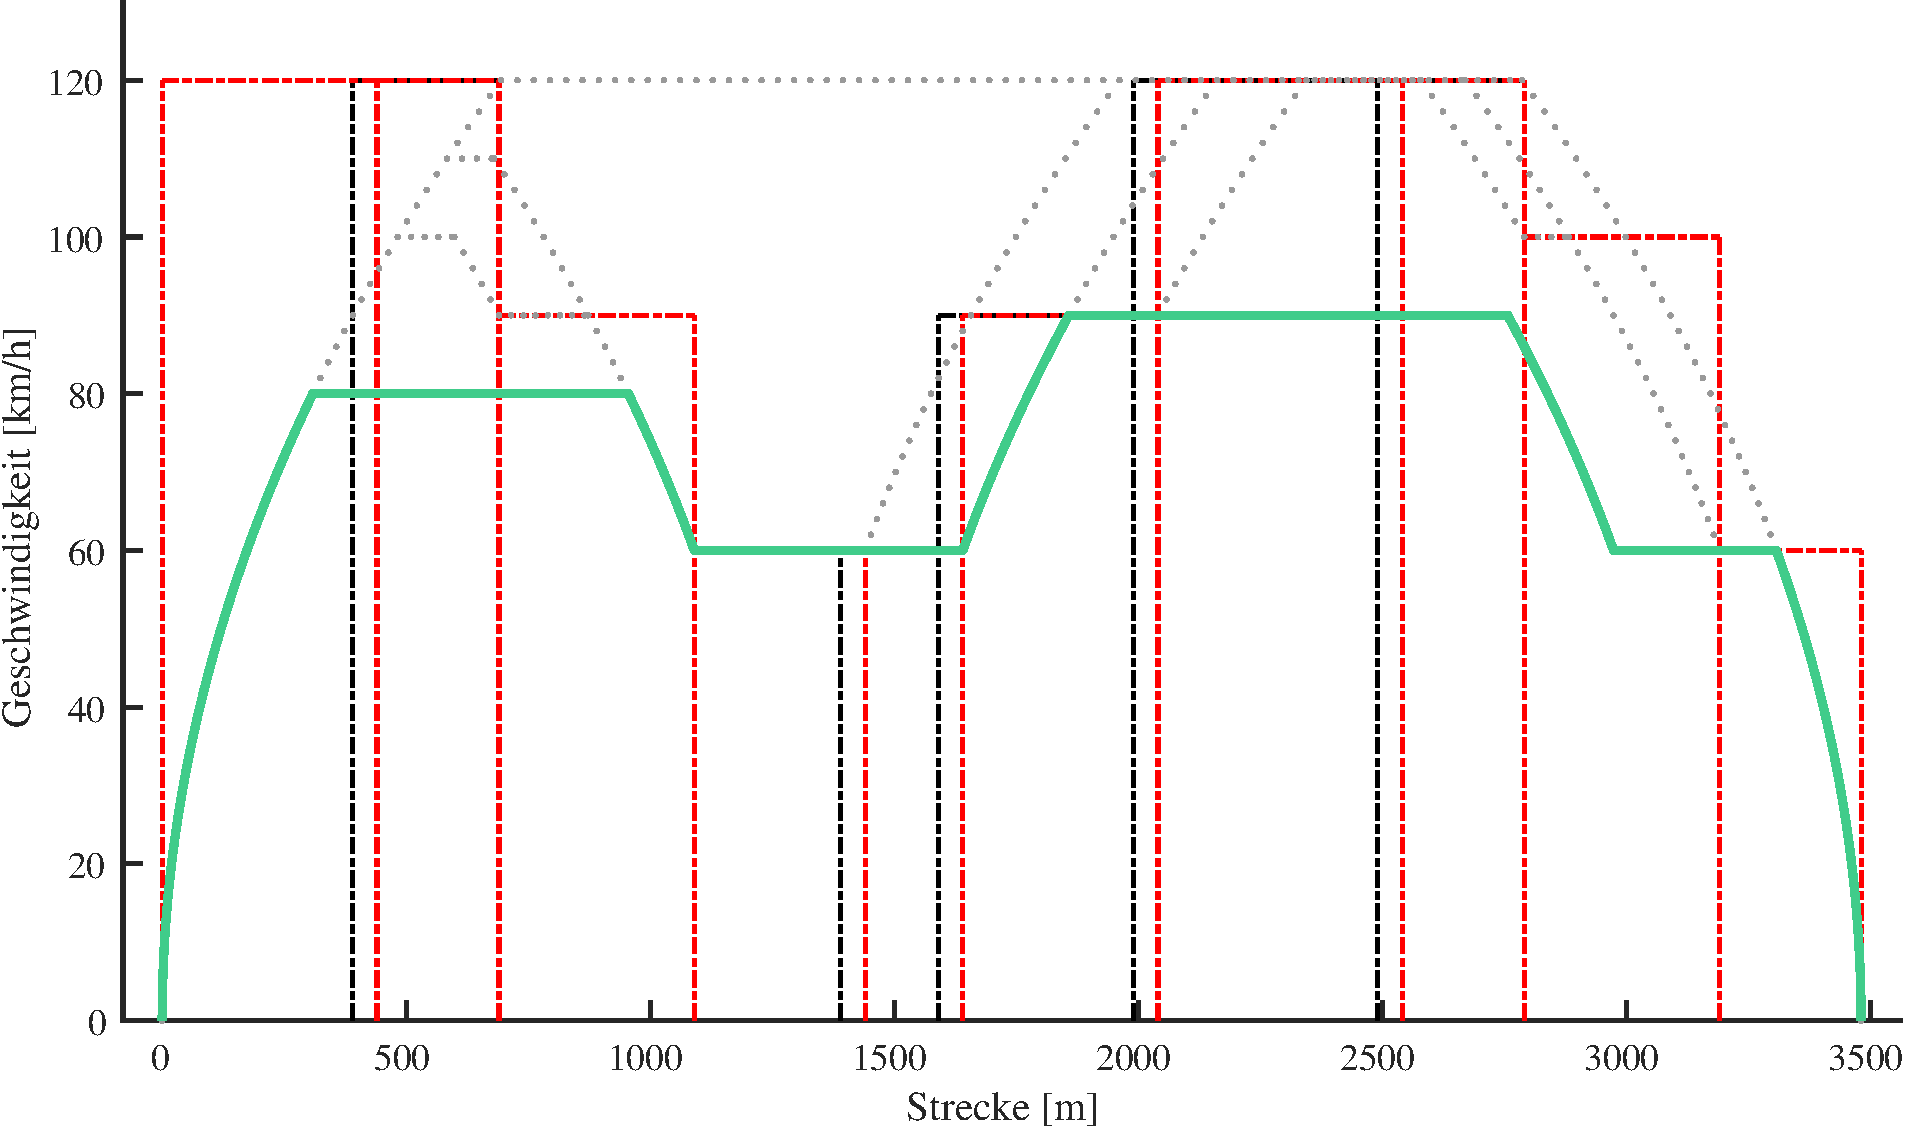
\includegraphics[width=\linewidth]{../images/matlab/it9.pdf}
\caption{\Gls{fahrtverlauf} unter Einhaltung der Mindestzeit}
\label{fig:it9}
\end{figure}
Für den Fall, dass das Fahrzeug auf einer Geschwindigkeit die Mindestzeit nicht einhält und als nächstes beschleunigen würde, kann die Beschleunigung später eingeleitet werden. 

\subsection{Berücksichtigung der Ankunftszeit bei der Berechnung des \Gls{fahrtverlauf}s} \label{time}
Der berechnete \Gls{fahrtverlauf} aus den Kapiteln \ref{v_max}, \ref{überprüfung}, \ref{neuberechnung} und \ref{minTime} ermittelt die frühstmögliche Ankunftszeit am Ziel. In dem Fall, dass der Zug dadurch mit einer Verspätung am Ziel ankommt, wird der \Gls{fahrtverlauf} an das Fahrzeug übergeben. Falls das Fahrzeug mit dem \Gls{fahrtverlauf} zu früh am Ziel ankommen würde, wird überprüft, ob es möglich ist die Geschwindigkeit zu reduzieren, sodass der Zug energieeffizienter fahren kann und ohne Verspätung am Ziel ankommt. 

Im ersten Schritt wird mittels der Funktion \textit{check\-If\-The\-Speed\-Can\-Be\-De\-creased$($$)$} (\textit{func\-tions\_""fahrt\-ver\-lauf\-.php}) überprüft, ob die Geschwindigkeit reduziert werden kann. Dabei werden alle \textit{\$keyPoints} ermittelt, bei denen das Fahrzeug beschleunigt und die beim darauffolgenden \textit{\$keyPoint} abbremsen. Für jeden dieser \textit{\$keyPoints} werden die möglichen Geschwindigkeiten ermittelt, welche das Fahrzeug zwischen den beiden \textit{\$keyPoints} fahren könnte. Für die Berechnung dieser Geschwindigkeiten wird als niedrigste Geschwindigkeit die \textit{speed\_0} des ersten \textit{\$keyPoints} bzw. \textit{speed\_1} des zweiten \textit{\$keyPoints} -- jenachdem, welche niedriger ist -- genommen und in 10 $km/h$-Schritten bis  \textit{speed\_1} des ersten \textit{\$keyPoints} abgespeichert. Daraus ergibt sich für jeden \textit{\$keyPoint} eine \textit{range} an möglichen Geschwindigkeiten. Als Rückgabewert der Funktion wird ein Array zurückgegeben, welches die Einträge \textit{possible} und \textit{range} enthält und als \textit{\$return\-Speed\-Decrease} abgespeichert. Der Eintrag \textit{possible} gibt an, ob das Fahrzeug auf dem gesamten \Gls{fahrtverlauf} die Geschwindigkeit reduzieren könnte und wird als Boolescher Wert (\textit{true}/\textit{false}) abgespeichert und in dem Array \textit{range} werden alle Indexe der möglichen \textit{\$keyPoints} inklusive der ermittelten Geschwindigkeiten abgespeichert.

In dem in Abbildung \ref{fig:it9} dargestellten \Gls{fahrtverlauf} wären für den \textit{\$keyPoint} mit dem Index 0 (die Indexe der \textit{\$keyPoints} entsprechen dem Zahlenbereich der $\mathbb{N}_0$) die Geschwindigkeiten 60, 70 und 80 $km/h$ ermittelt worden und für den \textit{\$keyPoint} mit dem Index 2 die Geschwindigkeiten 60, 70, 80 und 90 $km/h$.

Wenn eine Reduzierung der Geschwindigkeit möglich ist, wird in einer \textit{while}-Schleife versucht die Geschwindigkeit zu reduzieren, bis das Fahrzeug bei der nächsten Reduzierung mit einer Verspätung am Ziel ankommen würde oder eine weitere Reduzierung nicht möglich ist. Innerhalb der \textit{while}-Schleife ermittelt die Funktion \textit{find\-Max\-Speed$($$)$} (\textit{functions\_fahrtverlauf.php}) aus dem \textit{\$returnSpeedDecrease}-Array den \textit{\$keyPoint} mit der höchsten Geschwindigkeit. Für den Fall, dass mehrere \textit{\$keyPoints} die selbe Höchstgeschwindigkeit haben, wird der letzte dieser \textit{\$keyPoints} ermittelt. Im Anschluss wird mit einer \textit{for}-Schleife in 10 $km/h$-Schritten in absteigender Reihenfolge über die möglichen Geschwindigkeiten iteriert und überprüft, ob durch die Anpassung die Ankunftszeit eingehalten werden kann. Sobald die Ankunftszeit nicht eingehalten werden kann, werden die \textit{\$keyPoints} aus dem vorherigen Iterationsschritt gespeichert und die \textit{while}-Schleife wird abgebrochen. Sollte die \textit{for}-Schleife durchlaufen, ohne dass es zu einer Überschreitung der maximal verfügbaren Zeit kommt, wird die Funktion \textit{checkIfTheSpeedCanBeDecreased$($$)$} (\textit{functions\_fahrtverlauf.php}) erneut aufgerufen. 
Das Ergebnis dieser Berechnung ist in der Abbildung \ref{fig:it10} abgebildet.
\begin{figure}
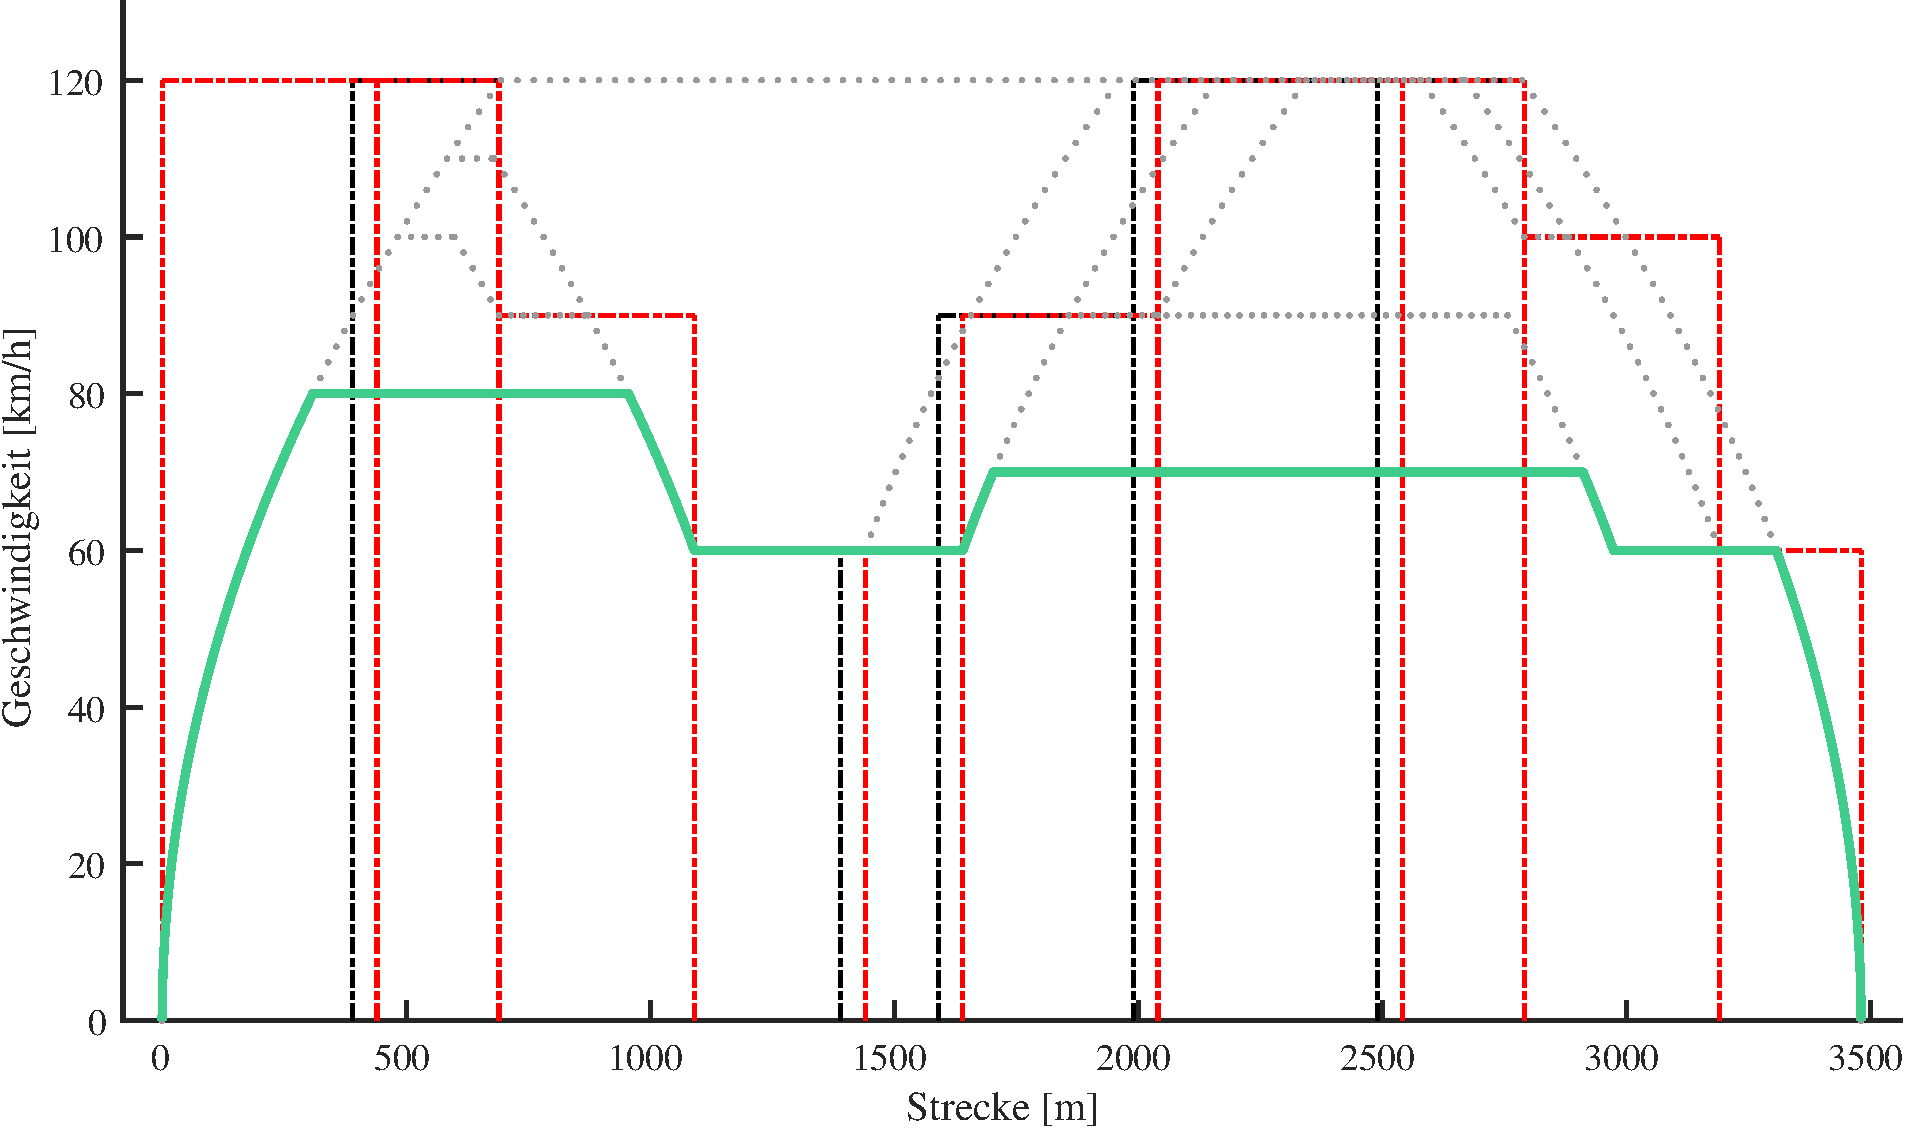
\includegraphics[width=\linewidth]{../images/matlab/it10.pdf}
\caption{\Gls{fahrtverlauf} mit reduzierter Geschwindigkeit unter Einhaltung der An\-kunfts\-zeit}
\label{fig:it10}
\end{figure}
\subsection{Berücksichtigung der exakten Ankunftszeit bei der Berechnung des \Gls{fahrtverlauf}s} \label{time2}
Die in Kapitel \ref{minTime} errechnete Ankunftszeit, beschreibt die spätmöglichste Ankunftszeit am Ziel, ohne dass das Fahrzeug mit einer Verspätung am Ziel ankommt, wenn bei einer Beschleunigung auf eine geringere Zielgeschwindigkeit beschleunigt wird. Dadurch wird das Fahrzeug im Normalfall nicht exakt pünktlich das Ziel erreichen. Über die Variable \textit{\$useSpeedFineTuning} kann festgelegt werden, ob das Fahrzeug eine exakte Ankunftszeit versuchen soll zu erreichen. Wenn diese Funktion aktiviert ist und der Eintrag \textit{possible} aus dem Array \textit{\$returnSpeedDecrease} \textit{true} ist, wird für den letzten \textit{\$keyPoint} aus dem \textit{\$return\-Speed\-De\-crease}-Array überprüft, ob die Verzögerung des nächsten \textit{\$keyPoints} vorzeitiger eingeleitet werden kann. Sollte die Zielgeschwindigkeit der Verzögerung 0 $km/h$ sein, wird die Verzögerung unterteilt in eine Verzögerung auf 10 $km/h$ und eine von 10 $km/h$ auf 0 $km/h$. Die Position der vorzeitig eingeleiteten Verzögerung wird mittels der Funktion \textit{speedFineTuning$($$)$} (\textit{functions\_fahrtverlauf.php}) berechnet, welche als Parameter den Betrag der Differenz zwischen aktueller Soll- und Ist-Ankunftszeit und den Index des vorherigen \textit{\$keyPoints} übergeben bekommt und auf der Gleichung \ref{eq:t_1_tuning} aus Kapitel \ref{formula} basiert.
\begin{figure}
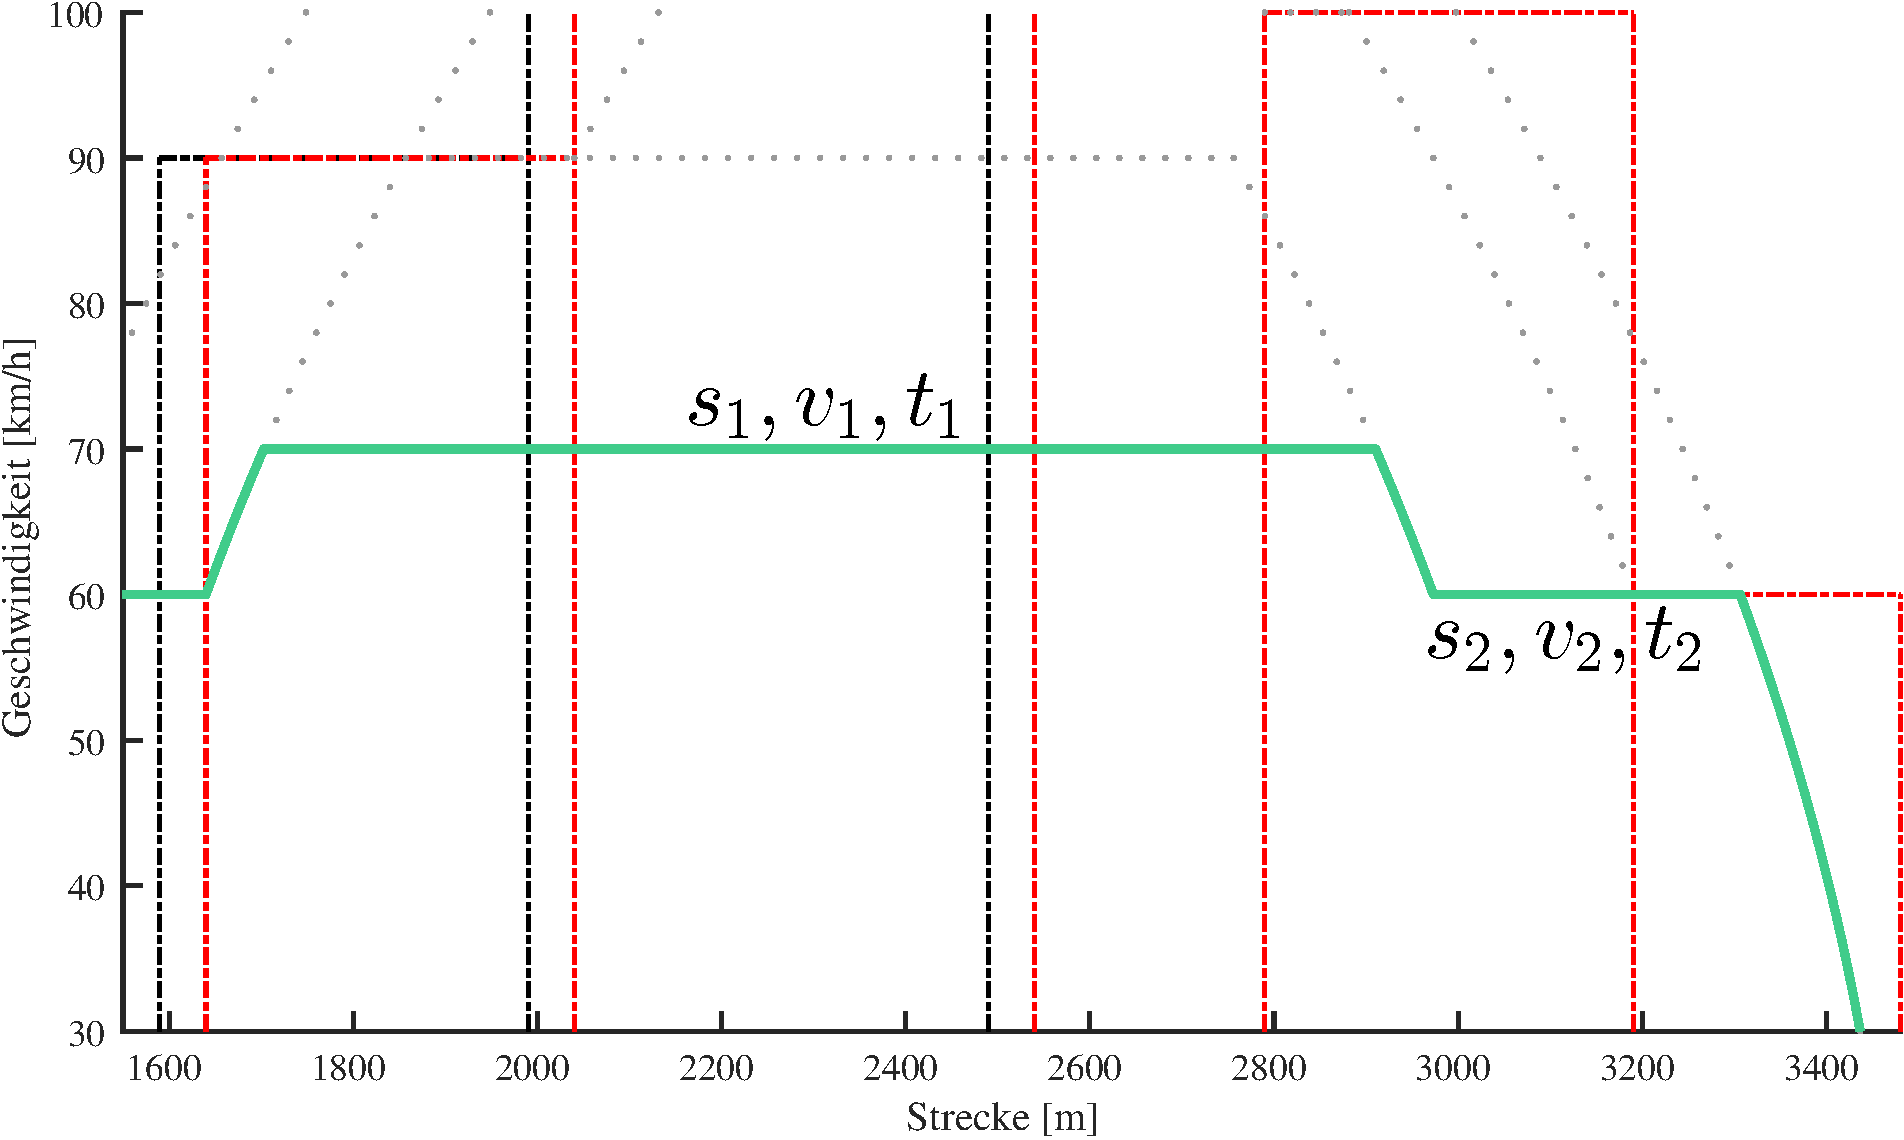
\includegraphics[width=\linewidth]{../images/matlab/it11.pdf}
\caption{\Gls{fahrtverlauf} vor der Anpassung der exakten Ankunftszeit}
\label{fig:it11}
\end{figure}
In Abbildung \ref{fig:it11} werden die Geschwindigkeiten ($v_1$, $v_2$), Strecken ($s_1$, $s_2$) und Zeiten ($t_1$, $t_2$) vor und nach der Verzögerung -- welche vorzeitiger eingeleitet werden soll, um eine pünktliche Ankunft am Ziel zu ermöglichen -- dargestellt und in Tabelle \ref{table:speed_fine_tuning_ex} sind die exakten Werte des exemplarischen \Gls{fahrtverlauf}s aufgelistet. In diesem konkreten Beispiel würde das Fahrzeug 3,31 $s$ ($t_{\varDelta}$) zu früh an der Betriebsstelle ankommen, wodurch das Fahrzeug für die Zurücklegung der Strecken $s_1$ und $s_2$ insgesamt 85,42 $s$ ($t_{ges}=t_1+t_2+t_{\varDelta}$) zur Verfügung hat.
\begin{table}
\begin{center}
\renewcommand{\arraystretch}{1.2}
\begin{tabular}{r l}
$v_1$                   &   70 $km/h$ ($\approx$ 19,44 $m/s$)                         \\ 
$v_2$                   &   60 $km/h$ ($\approx$ 16,67 $m/s$)                         \\ 
$s_1$                   &   1207,67 $m$                         \\ 
$s_2$                   &   333,33 $m$                         \\ 
$s_{ges}$                   &   1541 $m$                         \\ 
$t_1$                   &   62,11 $s$                         \\ 
$t_2$                   &   20 $s$                         \\ 
$t_{\varDelta}$                   &   3,31 $s$                         \\ 
$t_{ges}$                   &   85,42 $s$                         \\ 
\end{tabular}
\renewcommand{\arraystretch}{1}
\caption{Geschwindigkeiten, Strecken und Zeiten vor und nach der Verzögerung vor der Anpassung}
\label{table:speed_fine_tuning_ex}
\end{center}
\end{table}

Durch das Einsetzen der Werte in die Gleichung \ref{eq:t_1_tuning} aus dem Kapitel \ref{formulaGleichfoermig} ergibt sich für $t_3$ ($t_3$, $t_4$, $s_3$ und $s_4$ bezeichnen die Strecken und Zeiten nach der Anpassung) ein Wert von 42,2 $s$. Dementsprechend muss die Verzögerung 19,85 $s$ ($t_1$ - $t_3$) früher eingeleitet werden.
\begin{figure}[H]
\[t_{3} = \frac{1541\:m - 16,67\:m/s \cdot 85,42\:s}{19,44\:m/s - 16,67\:m/s}\]
%\[t_{3} = \frac{1541m - 1423,95 m}{2,77 m/s}\]
%\[t_{3} = \frac{117,05 m}{2,77 m/s}\]
\[t_{3} = 42,26\:s\]
\end{figure}
Die vorzeitige Einleitung der Verzögerung sorgt dafür, dass das Fahrzeug die nächste Betriebsstelle genau pünktlich erreicht und ist in Abbildung \ref{fig:it12} dargestellt, wobei durch die gepunktete Linie der \Gls{fahrtverlauf} vor der Anpassung zu sehen ist. Die neu berechneten Werte sind in Tabelle \ref{table:speed_fine_tuning_ex_2} aufgelistet.
\begin{figure}
  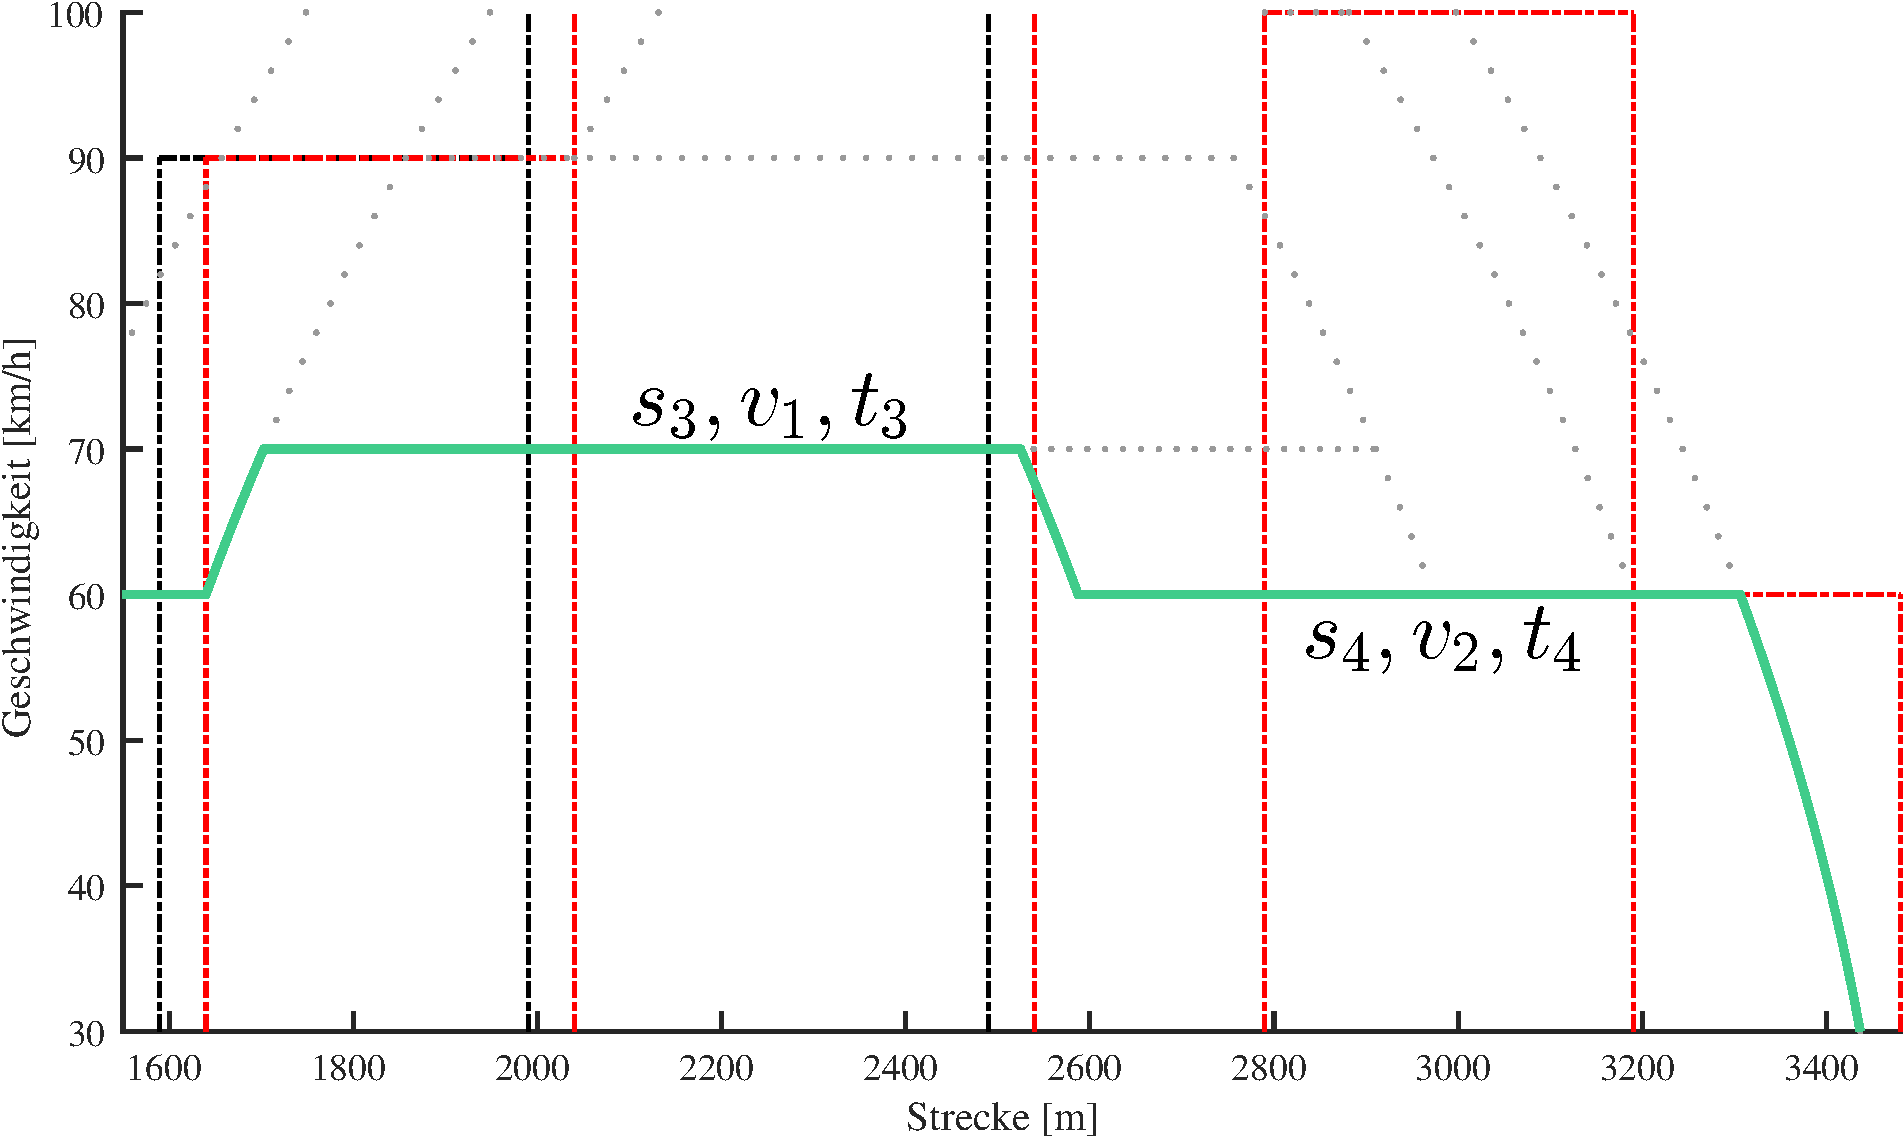
\includegraphics[width=\linewidth]{../images/matlab/it12.pdf}
  \caption{\Gls{fahrtverlauf} nach der Anpassung der exakten Ankunftszeit}
  \label{fig:it12}
\end{figure}
\begin{table}
\begin{center}
\renewcommand{\arraystretch}{1.2}
\begin{tabular}{r L{3cm}}
$s_3$                   	&   821,91 $m$                      	\\ 
$s_4$                   	&   719,1 $m$                         	\\ 
$t_3$                   	&   42,26 $s$                         	\\ 
$t_4$                   	&   43,16 $s$                         	\\ 
%$t_{ges}$           	&   85,42 $s$                         	\\ 
\end{tabular}
\renewcommand{\arraystretch}{1}
\caption{Geschwindigkeiten, Strecken und Zeiten vor und nach der Verzögerung nach der Anpassung}
\label{table:speed_fine_tuning_ex_2}
\end{center}
\end{table}
Der finale \Gls{fahrtverlauf} ist in Abbildung \ref{fig:it13} dargestellt und kann so dem Fahrzeug übergeben werden.
\begin{figure}
  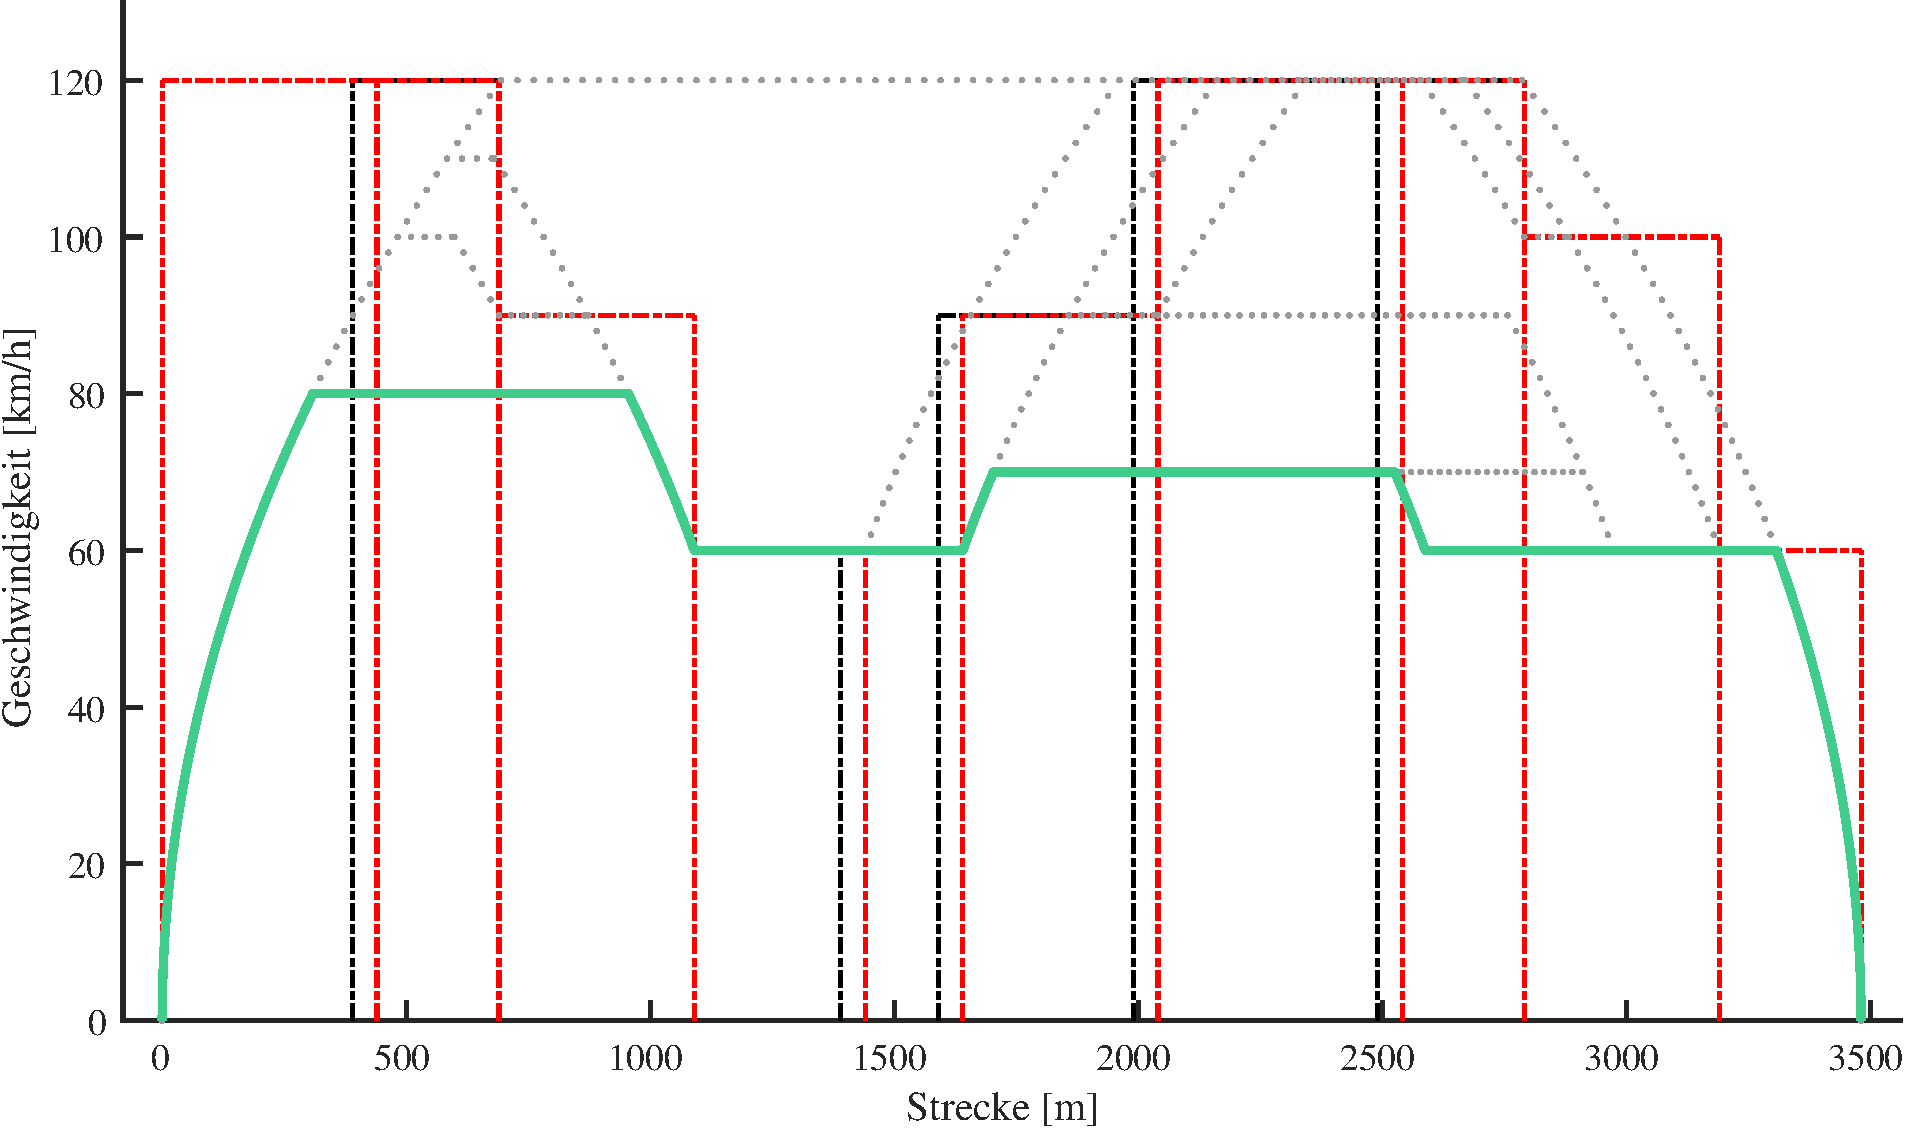
\includegraphics[width=\linewidth]{../images/matlab/it13.pdf}
  \caption{Ergebnis der \Gls{fahrtverlauf}s-Ermittlung}
  \label{fig:it13}
\end{figure}
\subsection{Einleitung einer Gefahrenbremsung} \label{notbremsung}
Eine Gefahrenbremsung wird eingeleitet, sobald ein Fahrzeug bei einer sofortigen Verzögerung ein auf Halt stehendes Signal überfahren würde, in einem \ac{infra} die zulässige Höchstgeschwindigkeit überschreiten würde oder an dem nächsten planmäßigen Halt nicht rechtzeitig zum stehen kommen würde. Bei einer Gefahrenbremsung wird mit einer Notbremsverzögerung von 2 $m/s^2$ abgebremst. Dieser Wert kann in der Datei \textit{global\_variables.php} über die Variable \textit{\$globalNotverzoegerung} angepasst werden. Für eine möglichst realitätsnahe Simulation einer Gefahrenbremsung, bei der das Risiko für Fahrzeugschäden möglichst gering ist, wurde sich dafür entschieden, dass die Fahrzeuge -- wenn sie an der Gefahrenstelle eine Geschwindigkeit haben, für die gilt: $v\geq$ 10 $km/h$ -- nach der Geschwindigkeit von 10 $km/h$ direkt die Geschwindigkeit von 0 $km/h$ übermittelt bekommen. Dadurch wird bei der Berechnung einer Gefahrenbremsung zwischen drei Fällen unterschieden:
\begin{enumerate}
\item Fahrzeug hält mit der Notbremsverzögerung vor der Gefahrenstelle
\item Fahrzeug hat bei der Gefahrenstelle eine Geschwindigkeit von $v<$ 10 $km/h$
\item Fahrzeug hat bei der Gefahrenstelle eine Geschwindigkeit von $v\geq$ 10$ km/h$
\end{enumerate}
Für die Überprüfung, ob das Fahrzeug mit der Notbremsverzögerung vor der Gefahrenstelle zum Stehen kommt, wird mittels der Funktion \textit{getBrakeDistance$($$)$} (\textit{functions.php}) der Bremsweg ($s_{Bremsweg}$) berechnet und mit der Distanz zur Gefahrenstelle ($s_{Gefahrenstelle}$) verglichen. Sollte für den Bremsweg gelten: $s_{Bremsweg}\leq s_{Gefahrenstelle}$, wird das Fahrzeug die Gefahrenbremsung einleiten und in 2 $km/h$-Schritten auf 0 $km/h$ abbremsen. In dem Fall, dass der Bremsweg länger als die Strecke bis zur Gefahrenstelle ist, wird überprüft, welche Geschwindigkeit das Fahrzeug an der Gefahrenstelle hat. Für diese Berechnung wird die Gleichung \ref{eq:gefahrenbremsung} aus dem Kapitel \ref{formulaBeschleunigung} verwendet. 

Sollte das Fahrzeug an der Gefahrenstelle eine Geschwindigkeit von $v\geq$ 10 $km/h$ haben, bremst das Fahrzeug in 2 $km/h$-Schritten auf 10 $km/h$ ab und bekommt nach der Übermittlung der 10 $km/h$ direkt 0 $km/h$ übergeben. In dem Fall, dass das Fahrzeug an der Gefahrenstelle langsamer als 10 $km/h$ ist, bremst das Fahrzeug wie im 1. Fall in 2 $km/h$-Schritten auf 0 $km/h$ ab. Bei einer Gefahrenbremsung bekommt das jeweilige Fahrzeug eine Fehlermeldung übermittelt und wird nicht weiterfahren, da durch die Gefahrenbremsung keine genaue Positionsbestimmung vorgenommen werden kann. Damit das Fahrzeug wieder seinen Fahrtbetrieb aufnehmen kann, muss das Fahrzeug händisch von der Anlage genommen werden, gewartet werden, bis die Fahrzeugsteuerung das Entfernen registriert hat und wieder neu positioniert werden.
\newpage
\section{Formeln} \label{formula}
\begin{flushleft}
Für die im folgenden Kapitel verwendeten Einheiten gilt:
\end{flushleft}

\begin{centering}
\begin{conditions}
a     &  Bremsverzoegerung [$m/s^{2}$] \\
v     &  Geschwindigkeit [$m/s$] \\
s     &  Strecke [$m$] \\
t     &  Zeit [$s$]
\end{conditions}
\end{centering}
\subsection{Formeln für gleichmäßig beschleunigte Bewegungen} \label{formulaBeschleunigung}
\noindent Bei einer gleichmäßig beschleunigten Bewegung gilt:\footnote{\citet[S. 22]{richard2011technische}}
\begin{equation}
a(t) = a
\end{equation}
Für die Bestimmung der Geschwindigkeit in Abhängigkeit der Zeit, muss die Beschleunigung $a(t)$ nach der Zeit $t$ integriert werden.\footnote{\citet[S. 20]{richard2011technische}}
\begin{equation}
v(t) = \int a(t) \,dt
\end{equation}
Daraus ergibt sich folgende Gleichung für die Geschwindigkeit in Abhängigkeit der Zeit. Die bei der Integration entstehende Integrationskonstante $v_{0}$ gibt dabei die Startgeschwindigkeit an.
\begin{equation}
v(t) = a \cdot t + v_{0}
\end{equation} %\footnote{ebd. (S. 20)}
Für die Bestimmung der benötigten Zeit muss die Geschwindigkeit erneut integriert werden.\footnote{\citet[S. 20]{richard2011technische}} Die dabei entstehende Integrationskonstante $s_{0}$ gibt die bereits zurückgelegte Strecke an.
\begin{equation}
s(t) = \int v(t) \,dt
\end{equation}
\begin{equation}
s(t) =\frac{1}{2} \cdot a \cdot t^{2} + v_{0}  \cdot t + s_{0}
\end{equation}
Bei der Verwendung dieser Gleichung werden die Integrationskonstanten $v_{0}$ und $s_{0}$ gleich $0$ gesetzt, damit die Gleichungen allgemein gültig sind. Für die Berechnung des Beschleuniguns- und Abbremsverhalten der Fahrzeuge ist es notwendig zu wissen, welche Strecke ein Fahrzeug zurücklegen muss, um von einer Startgeschwindigkeit $v_{0}$ auf eine Zielgeschwindigkeit $v_{1}$ zu beschleunigen bzw. abzubremsen. Dafür wird die Gleichung für die Geschwindigkeit $v(t)$ nach $t(v)$ umgestellt und und in die Gleichung $s(t)$ eingesetzt. Daraus ergibt sich folgende Gleichung für die Strecke in Abhängigkeit von der Geschwindigkeit:
\begin{equation}
t(v) = \frac{v}{a}
\end{equation}
\begin{equation}
s(v) =\frac{1}{2} \cdot \frac{v^{2}}{a}
\end{equation}
Durch die Festlegung von $v_{0} = 0$ wird so die benötigte Strecke ermittelt, welche ein Fahrzeug bei einer gegebenen Bremsverzögerung $a$ benötigt, um von 0 $m/s$ auf eine gegebenen Zielgeschwindigkeit $v_{1}$ zu beschleunigen. Bei der Berechnung des Beschleuniguns- und Abbremsverhalten wird es aber auch zu Situationen kommen, bei denen ein Fahrzeug eine Startgeschwindigkeit hat, für die gilt $v_{0} \neq 0$. Um eine allgemein gültige Gleichung aufzustellen, wird für die Ermittlung der benötigten Strecke bei einer gegebenen Start- und Zielgeschwindigkeit die Strecke berechnet, die das Fahrzeug benötigt, um von 0 $m/s$ auf $v_{1}$ und von 0 $m/s$ auf $v_{0}$ zu beschleunigen. Für die gesuchte Strecke gilt dann: 
\begin{equation}
s(v_{0}, v_{1}) = \abs{s(v_{1}) - s(v_{0})} 
\end{equation}
\begin{equation}
\label{eq:s_v_ges}
s(v_{0}, v_{1}) =\frac{1}{2} \cdot\abs{\frac{v_{1}^{2} - v_{0}^{2}}{a}}
\end{equation}
In der Fahrzeugsteuerung übernimmt diese Berechnung die Funktion \textit{getBrakeDistance()} (Code-Beispiel \ref{lst:getBrakeDistance}). 
\begin{figure}[H]
\begin{lstlisting}[caption={\textit{getBrakeDistance$($$)$} (\textit{functions\_math.php})},captionpos=b,label={lst:getBrakeDistance}]
// Ermittlung der Strecke für eine Beschleunigung bzw. Verzögerung
function getBrakeDistance (float $v_0, float $v_1, float $verzoegerung) {
	return abs(0.5 * ((pow($v_0/3.6,2) - pow($v_1/3.6, 2))/($verzoegerung)));
}
\end{lstlisting}
\end{figure}
\noindent Neben der Berechnung der Strecke ist auch die benötigte Zeit essenziell. Dafür wird mittels $t(v)$ die Zeit berechnet, die das Fahrzeug benötigt, um von 0 $km/h$ auf $v_{0}$ bzw. $v_{1}$ zu beschleunigen und aus der Differenz wird die benötigte Zeit berechnet.
\begin{equation}
\label{eq:t_v_ges}
t(v_{0}, v_{1}) = \abs{\frac{v_{1} - v_{0}}{a}}
\end{equation}
In der Fahrzeugsteuerung übernimmt diese Berechnung die Funktion \textit{getBrakeTime()} (\textit{func\-tions\_""math\-.php}) (Code-Beispiel \ref{lst:getBrakeTime}).
\begin{figure}[H]
\begin{lstlisting}[caption={\textit{getBrakeTime$($$)$} (\textit{functions\_math.php})},captionpos=b,label={lst:getBrakeTime}]
// Ermittelt die Distanz für Brems- und Verzögerungsvorgänge
function getBrakeTime (float $v_0, float $v_1, float $verzoegerung) {
	return abs((($v_1/3.6)/$verzoegerung) - (($v_0/3.6)/$verzoegerung));
}
\end{lstlisting}
\end{figure}
\noindent Für die Berechnung einer Gefahrenbremsung ist es notwendig zu wissen, welche Geschwindigkeit das Fahrzeug an der Position der Gefahrenstelle hat. Dafür wird die Gleichung \eqref{eq:s_v_ges} nach $v_{2}$ umgestellt. Umgesetzt wird diese Gleichung mit der Funktion \textit{get\-Tar\-get\-Brake\-Speed\-With\-Dis\-tance\-And\-Start\-Speed$($$)$} (\textit{func\-tions\_""math\-.php}) (Code-Beispiel \ref{lst:getTargetBrakeSpeedWithDistanceAndStartSpeed}).
\begin{equation}
\label{eq:gefahrenbremsung}
v_{2}(v_{1}, s) = \sqrt{-2 \cdot s \cdot a} + v_{1}
\end{equation}
\begin{figure}[H]
\begin{lstlisting}[caption={\textit{getTargetBrakeSpeedWithDistanceAndStartSpeed$($$)$} (\textit{func\-tions\_""math\-.php})},captionpos=b,label={lst:getTargetBrakeSpeedWithDistanceAndStartSpeed}]
// Ermittelt die Geschwindigkeit, die ein Fahrzeug in einem Bremsvorgang
// nach einer gegebenen Distanz hat.
function getTargetBrakeSpeedWithDistanceAndStartSpeed (float $distance, float $verzoegerung, int $speed) {
	return sqrt((-2 * $verzoegerung * $distance) + (pow(($speed / 3.6), 2)))*3.6;
}
\end{lstlisting}
\end{figure}
\subsection{Formeln für gleichförmige Bewegungen} \label{formulaGleichfoermig}
Bei einer gleichförmigen Bewegung gilt der Grundsatz:\footnote{\citet[S. 22]{richard2011technische}}
\begin{equation}
v(t) = v
\end{equation}
Für die Berechnung der Strecke gilt wie bei der gleichmäßig beschleunigten Bewegung:\footnote{\citet[S. 20]{richard2011technische}}
\begin{equation}
s(t) = \int v(t) \,dt
\end{equation}
\begin{equation}
s(t) =v \cdot t + s_{0}
\end{equation}
Damit die Gleichung allgemeingültig ist, wird die Integrationskonstante $s_{0}$ gleich 0 gesetzt.
\begin{equation}
s(t) =v \cdot t
\label{eq:s_v_t}
\end{equation}
\begin{figure}[H]
\begin{lstlisting}[caption={\textit{distanceWithSpeedToTime$($$)$} (\textit{functions\_math.php})},captionpos=b,label={lst:distanceWithSpeedToTime}]
// Ermittelt die Zeit, die ein Fahrzeug bei einer gegebenen Strecke für
// eine gegebene Distanz benötigt
function distanceWithSpeedToTime (int $v, float $distance) {
	return (($distance)/($v / 3.6));
}
\end{lstlisting}
\end{figure}
\noindent Für die Einhaltung der exakten Ankunftszeit, muss errechnet werden, wie lange das Fahrzeug bei zwei gegebenen Geschwindigkeiten ($v_1$ und $v_2$) auf den jeweiligen Geschwindigkeiten fahren muss, um die Gesamtstrecke ($s_{ges}$) und die Gesamtzeit ($t_{ges}$) einzuhalten. Für die Zeiten und Strecken gilt:
\begin{equation}
\label{eq:t_ges}
t_{ges} = t_{1} + t_{2}
\end{equation}
\begin{equation}
\label{eq:s_ges}
s_{ges} = s_{1} + s_{2}
\end{equation}
Durch das Einsetzen der Gleichung \eqref{eq:s_v_t} in die Gleichung \eqref{eq:s_ges} erhält man folgende Gleichung:
\begin{equation}
\label{eq:s_ges_2}
s_{ges} = v_{1} \cdot t_{1} + v_{2} \cdot t_{2}
\end{equation}
Durch das Umstellen der Gleichung \eqref{eq:t_ges} nach $t_{2}$ und dem Einsetzen in Gleichung \eqref{eq:s_ges_2} gilt für $t_{1}$:
\begin{equation}
\label{eq:t_1_tuning}
t_{1} = \frac{s_{ges} - v_{2} \cdot t_{ges}}{v_{1} - v_{2}}
\end{equation}
\begin{figure}[H]
\begin{lstlisting}[caption={\textit{calculateDistanceforSpeedFineTuning$($$)$} (\textit{functions\_math.php})},captionpos=b,label={lst:calculateDistanceforSpeedFineTuning}]
// Ermittelt die Distanz, um die eine Verzögerung "verschoben" werden müsste,
// damit die exakte Ankunftszeit eingehalten werden kann.
function calculateDistanceforSpeedFineTuning(int $v_0, int $v_1, float $distance, float $time) : float {
	return $distance - (($distance - $time * $v_1 / 3.6)/($v_0 / 3.6 - $v_1 / 3.6)) * ($v_0 / 3.6);
}
\end{lstlisting}
\end{figure}
%\begin{forest}
  for tree={
    font=\ttfamily,
    grow'=0,
    child anchor=west,
    parent anchor=south,
    anchor=west,
    calign=first,
    edge path={
      \noexpand\path [draw, \forestoption{edge}]
      (!u.south west) +(7.5pt,0) |- node[fill,inner sep=1.25pt] {} (.child anchor)\forestoption{edge label};
    },
    before typesetting nodes={
      if n=1
        {insert before={[,phantom]}}
        {}
    },
    fit=band,
    before computing xy={l=15pt},
  }
[project
  [php
    [main.php]
    [functions
    	[sort\_functions.php]
	[time\_functions.php]
    ]
    [database
    	[load\_trains.php]
    ]
  ]
  [matlab
    [plot\_v\_over\_distance.m]
  ]
  [latex
  	[paper.tex]
	[paper.bib]
	[fazit.tex]
	[grundlagen.tex]
	[paper.tex]
  ]
]
\end{forest}
%\newpage
\appendix
\newpage

\section{Anhang}

\subsection{fahrzeugsteuerung.php} \label{anhangMain}

\lstinputlisting[language=php,nolol]{../php/fahrzeugsteuerung.php}

\newpage

\subsection{functions.php} \label{sortFunctions}

\lstinputlisting[language=php,nolol]{../php/functions/functions.php}

\newpage

\subsection{functions\_fahrtverlauf.php} \label{fahrtverlaufFunctions}

\lstinputlisting[language=php,nolol]{../php/functions/functions_fahrtverlauf.php}

\newpage

\subsection{functions\_math.php} \label{functionsMath}

\lstinputlisting[language=php,nolol]{../php/functions/functions_math.php}

\newpage

\subsection{functions\_cache.php} \label{cacheFunctionsOwn}

\lstinputlisting[language=php,nolol]{../php/functions/functions_cache.php}

\newpage

\subsection{functions\_db.php} \label{functionsDatabase}

\lstinputlisting[language=php,nolol]{../php/functions/functions_db.php}

\newpage

\subsection{global\_variables.php} \label{anhangGlobalVariables}

\lstinputlisting[language=php,nolol]{../php/global_variables.php}

\newpage

\subsection{speed\_over\_position.m} \label{anhangMatlab}

\lstinputlisting[language=matlab,nolol]{../matlab/speed_over_position.m}

\newpage
\pagenumbering{Roman} % roman pagenumbers
\setcounter{page}{4}
\bibliography{paper}  % implement the name of the bibtex.bib file
\end{document}